\documentclass[diss,capa]{texufpel}

\usepackage[utf8]{inputenc}
\usepackage{graphicx}
\usepackage[T1]{fontenc}

\hypersetup{
    hidelinks,
    unicode=true,
    linktoc=all
}

\unidade{Centro de Desenvolvimento Tecnológico}
\programa{Programa de Pós-Graduação em Computação}
\curso{Ciência da Computação}

\unidadeeng{Technology Development Center}
\programaeng{Postgraduate Program in Computing}
\cursoeng{Computer Science}

\title{Aplicação de Técnicas de Mineração de Dados e Learning Analytics para Predição de Evasão de Alunos na UFPel}

\author{Costa}{Alexandre Gomes da}
\advisor[Prof.~Dr.]{Mattos}{Julio Carlos Balzano de}
\coadvisor[Prof.~Dr.]{Primo}{Tiago Thompsen}
% \collaborator[Prof.~Dr.]{Aguiar}{Marilton Sanchotene de}

%Palavras-chave em PT_BR
\keyword{mineração de dados educacionais}
\keyword{learning analytics}
\keyword{técnicas de predição}
\keyword{kdd}
\keyword{descoberta de conhecimento em base de dados}

%Palavras-chave em EN_US
\keywordeng{educational data mining}
\keywordeng{learning analytics}
\keywordeng{prediction techniques}
\keywordeng{kdd}
\keywordeng{knowledge-discovery in databases}

\begin{document}

\maketitle 

\sloppy

\fichacatalografica

%Composição da Banca Examinadora
\begin{aprovacao}{01 de agosto de 2020} %data da banca por extenso
\noindent Prof. Dr. Julio Carlos Balzano de Mattos (orientador)\\
Doutor em Computação pela Universidade Federal do Rio Grande do Sul.\\[1cm]

\noindent Prof. Dr. Tiago Thompsen Primo\\
Doutor em Computação pela Universidade Federal do Rio Grande do Sul.\\[1cm]

\noindent Prof. Dr. Ricardo Matsumura Araujo\\
Doutor em Computação pela Universidade Federal do Rio Grande do Sul.\\[1cm]

\noindent Prof. Dr. Luciano da Silva Pinto\\
Doutor em Biotecnologia pela Universidade Federal de Pelotas.
\end{aprovacao}

%Opcional
\begin{dedicatoria}
  Dedico\ldots 
\end{dedicatoria}

%Opcional
\begin{agradecimentos}
  Agradeço\ldots 
\end{agradecimentos}

%Opcional
\begin{epigrafe}
  Tudo o que não puder contar como fez; Não o faça! Se há razões para não contar; há para não o fazer.\\
  {\sc --- Kant}
\end{epigrafe}

%Resumo em Portugues (no maximo 500 palavras)
\begin{abstract}
 Os sistemas de gestão para educação armazenam uma grande quantidade de dados oriundos de diversas modalidades de interação entre alunos e professores mas também entre os alunos e o ambiente educacional. Analisar e encontrar padrões nesta quantidade de dados manualmente é inviável, por isso a utilização de Mineração de Dados Educacionais (MDE) é largamente utilizada. Este trabalho apresenta modelos de predição de alunos em risco de evasão usando apenas os dados dos três primeiros semestres cursados pelos alunos (N=1516) no curso de Ciência da Computação da Universidade [Blind]. Neste trabalho é utilizada a metodologia CRISP-DM e os dados extraídos no sistema acadêmico [Blind]. São apresentados resultados para três algoritmos e sendo que para o \textit{Logistic Regression} o resultado obtido foi um \textit{precision} de 91,24\% e um \textit{Recall} de 92,17\%, indicando que é possível criar um modelo de predição utilizando apenas os dados dos três primeiros semestre.
\end{abstract}

%Resumo em Inglês (no maximo 500 palavras)
\begin{englishabstract}{Application of Data Mining Techniques and Learning Analytics for Student Dropout Prediction at UFPel}
Educational Management Systems store a large amount of data from interaction of not only students and professors but also of students and the educational environment. Analyze and find patterns manually from a huge amount of data is hard, so Educational Data Mining (EDM) is widely used. This work presents a model that can predict the student's risk of dropout using data from the first three semesters attended by Computer Science Undergraduate students (N=1516) from University [Blind]. This work uses the CRISP-DM methodology e data from [Blind] Management System. The results are shown for three algorithms and for the Logistic Regression algorithm a precision of 91.24\% and a Recall of 92.17\% is presented indicating that it is possible to use a prediction model using only the data from the first three semesters of the course. from Pellets.
\end{englishabstract}

%Lista de Figuras
\listoffigures

%Lista de Tabelas
\listoftables

%lista de abreviaturas e siglas
\begin{listofabbrv}{ABNT}%coloque aqui a maior sigla para ajustar a distância
        \item[ABNT] Associação Brasileira de Normas Técnicas
        \item[NUMA] Non-Uniform Memory Access
        \item[SIMD] Single Instruction Multiple Data
        \item[SMP] Symmetric Multi-Processor
        \item[SPMD] Single Program Multiple Data
\end{listofabbrv}

%Sumario
\tableofcontents

\chapter{Introdução}

O uso constante de Tecnologia da Informação e Comunicação em diversas áreas vêm gerando um grande volume de dados.
Tecnologias como a internet, redes sociais, ambientes virtuais de aprendizagem, dispositivo móveis, aplicativos embarcados, leitores de código de barras, sensores, leitores biométricos e sistemas de informação em geral são alguns exemplos de recursos que vem aumentando o número de dados das mais diversas naturezas \cite{goldschmidt2015data}.

%% Educação
Atualmente, as áreas como a educação produzem uma grande quantidade de dados relacionados a alunos e professores todos os dias.
Para isto, esta área utiliza sistemas para fazer o controle de iterações acadêmicas, gestão de projetos de pesquisa, ensino ou extensão, ou até mesmo sistemas para fazer o controle de gestão de pessoas são alguns do exemplos de sistemas que podem gerar um volume considerável de dados.

A partir desse volume de dados é possível analisar problemas recorrentes relacionados a educação.
Um desses problemas é a evasão escolar que ainda é um desafio a ser superado.
A evasão é um problema que atinge não só as Instituições de Ensino Superior (IES) privadas, mas também as públicas.
Segundo dados do \citet{inep:2018}, em 2017, o índice de matrículas desvinculadas em todo o Brasil foi de 16,41\%.
Já para as IES públicas esse índice no mesmo período foi de 11,56\%.
Outro valor a ser considerado é o número de matriculas trancadas, onde foi de 11,17\% em todo o Brasil e 8,10\% IES públicas.

Comparando os índices da Universidade Federal de Pelotas (UFPel) com os do \citet{inep:2018} estes índices não mudam muito.
Em 2017 o índice de matriculas desvinculadas na UFPel foi de de 11,53\% que está abaixo do índice de 11,56\% apresentado pelo \citet{inep:2018}.
Mas olhando para a evasão curso a curso no ano de 2017 observamos dados alarmantes.
Por exemplo, temos cursos como o de Geoprocessamento onde a taxa de evasão semestral foi de 29,07\%.
Esse fenômeno é conhecido na estatística como paradoxo de Simpson, uma tendência aparece em um determinado grupo de dados e desaparece quando estes dados são combinado.
Ou seja, olhando para os cursos individualmente vários deles apresentam uma taxa de evasão bem elevada, mas quando essas taxas são combinadas a taxa de evasão não é tão relevante \cite{wagner1982simpson}.
Olhando para esses dados algumas perguntas surgem tais como ``Qual é o perfil do aluno que tende a evadir?'' ou ``Qual é a quantidade de alunos que trancaram e acabaram evadindo?'', por exemplo.

%% Knowledge Discovery in Database - KDD
Embora com ajuda de ferramentas computacionais, analisar essa crescente quantidade de dados não é trabalho para o homem \cite{goldschmidt2015data}.
Para ajudar nesta questão a área de Descoberta de Conhecimento em Base de Dados (\textit{Knowledge Discovery in Database} - KDD) é focada em extrair conhecimento encima de granes volumes de dados.
O termo mais conhecido relacionado a essa área é a Mineração de Dados (MD) que é uma das etapas do processo de KDD.

%% Mineração de dados educacionais
Segundo \citet{Koedinger2008} Mineração de Dados (MD) aplicada à educação é um campo interdisciplinar emergente mais conhecido como Mineração de Dados Educacionais (MDE).
\citet{baker2010data} define MDE como a área de investigação científica centrada no desenvolvimento de métodos para fazer descobertas dentro dos tipos de dados que vêm de ambientes educacionais e usando esses métodos para entender melhor os alunos e a aprendizagem deles.
A Figura \ref{fig:areas-relacionadas-mde} mostra que a área de MDE pode ser a combinação de 3 grandes áreas (ciência da computação, estatistia e educação) e serve de exemplo para justificar a interdisciplinaridade da área.

\begin{figure}[htbp]
    \centering 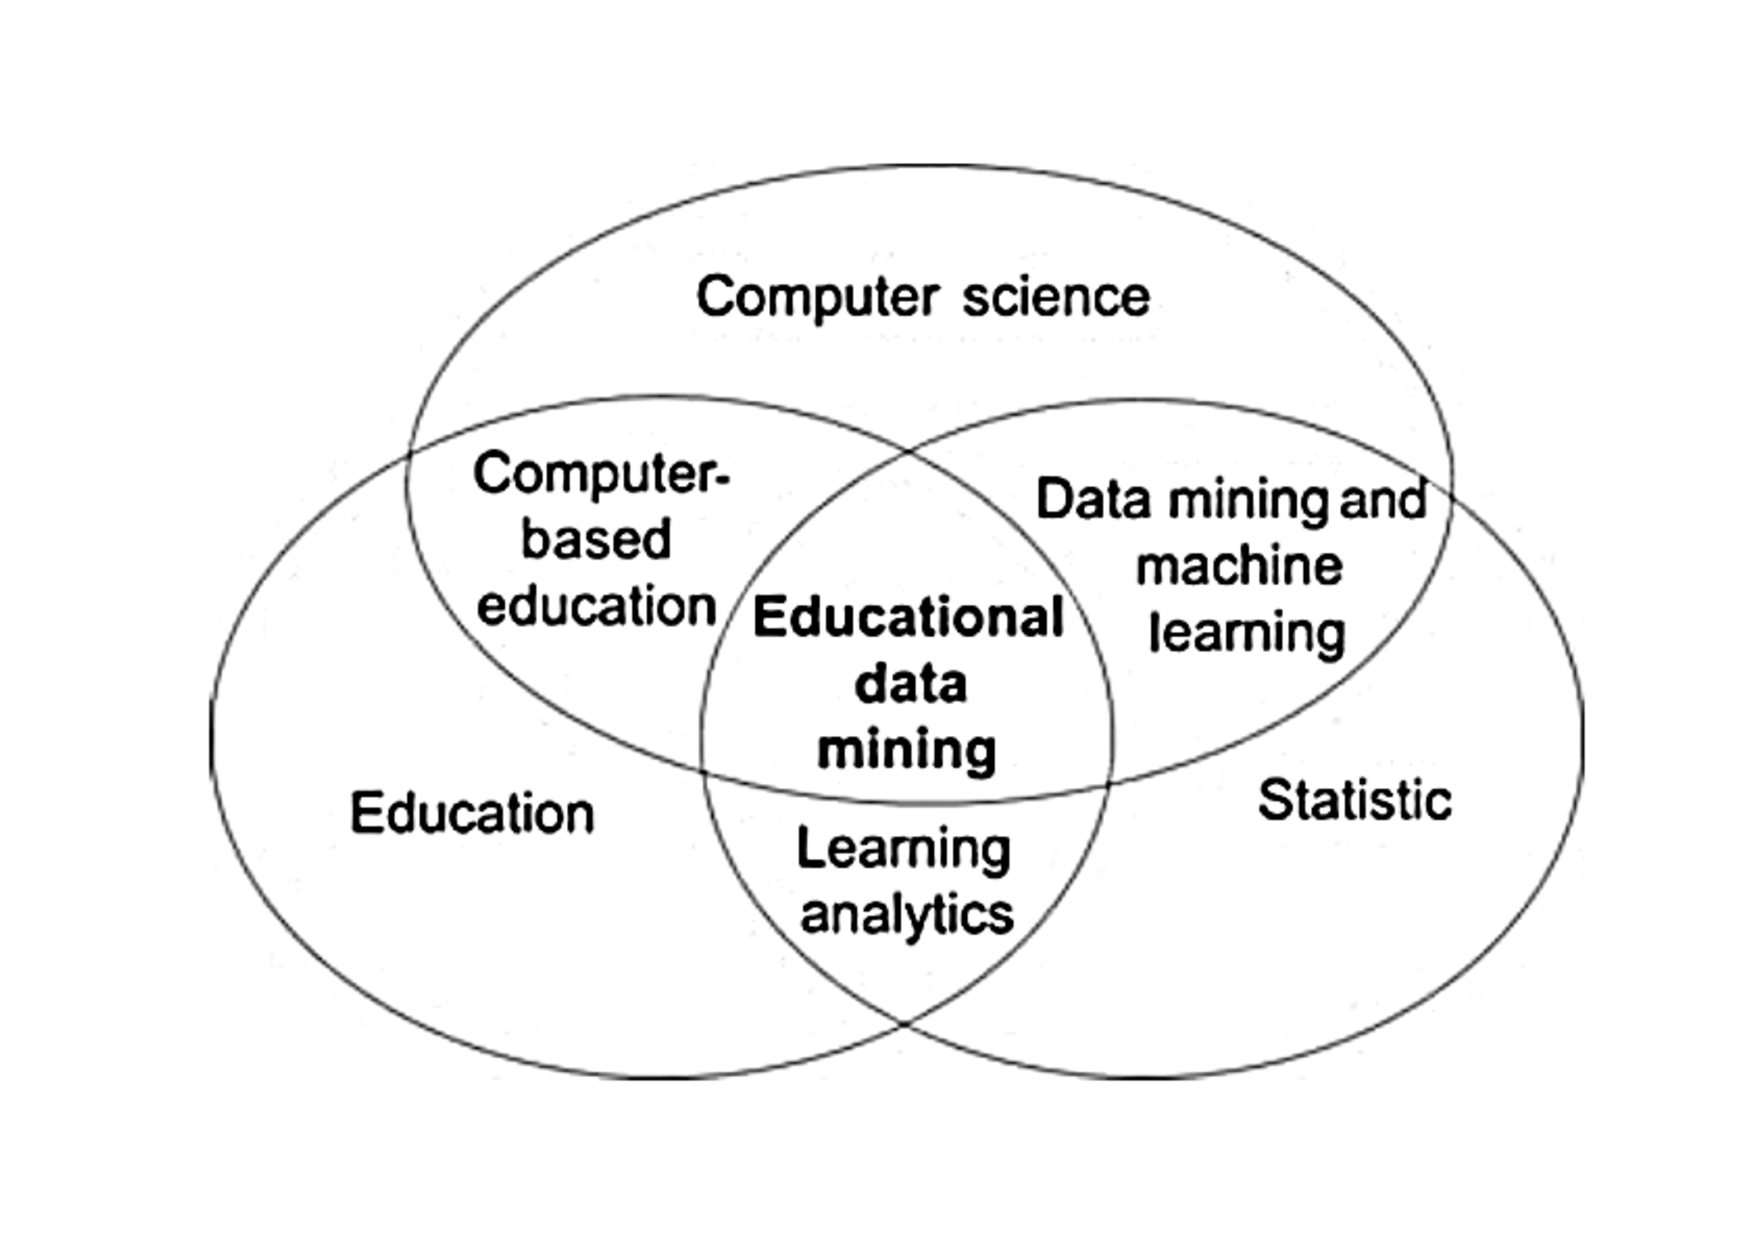
\includegraphics[scale=.4]{imagens/areas-edm.pdf}
    \caption{Principais áreas relacionadas com mineração de dados educacionais. \cite{Koedinger2008}}
    \label{fig:areas-relacionadas-mde}
\end{figure}

Neste trabalho iremos explorar a utilização de MDE/LA visando classificar e identificar perfis de alunos com tendência a evadir.
Segundo \citet{goldschmidt2015data} uma tarefa de classificação possui dois grupos.
Um grupo contem normalmente um atributo apenas que vai servir para fazer a predição de um valor (atributo-alvo).
Outro grupo corresponde aos atributos que vão servir para fazer a predição do valor (atributos de predição).
Tarefas de classificação são largamente utilizadas para fazer a predição de alunos em risco de evasão escolar, como será apresentado nesta proposta.

\citet{baker2010data} agrupa o problema de evasão em uma categoria ou tarefa de detectar o comportamento do aluno.
Onde o objetivo é detectar os alunos que têm algum tipo de problema ou comportamento incomum, por exemplo: pouca motivação, trapaça, evasão escolar, etc.
Destaca também que as principais técnicas usadas para resolver esses tipos de problemas são de classificação e agrupamentos.

%% Justificativa
Este trabalho possui como motivação o grande problema de evasão encontrado nos cursos superiores, em especial em alguns cursos sendo principalmente cursos das engenharias e exatas, e a dificuldade de traçar o perfil destes alunos.
Além disso, existe uma enorme quantidade de dados históricos de cursos de graduação presencias da UFPEL, uma vez que a grande maioria dos trabalhos vem de cursos EAD.
Quanto alguns trabalhos fazem questionários, provas, exercícios, etc, no presente trabalho serão coletado dados que foram gerados a partir de resultado que os alunos obtiveram em diversas disciplinas, cursos entre outros.
Este trabalho utilizará a base de dados do Sistema Integrado de Gestão da UFPEL (Cobalto).
A base do Cobalto conta também com os dados históricos do GOL que foi o sistema acadêmico da UFPEL de 2006 à 2013.

Este trabalho apresenta a investigação dos motivos que levam o alunos evadir com ajuda de técnicas de MDE através dos dados acadêmicos dos alunos do curso de Ciência da Computação da Universidade [Blind] que foi escolhido preliminarmente por possuir elevados índices de evasão. Para este propósito, foi analisado e coletado dados dos 3 primeiros semestres de alunos do curso de 2000 a 2020, para responder as seguintes questões de pesquisa: (Q1) Quais são os atributos que mais influenciam no processo de evasão dos estudantes em cursos de computação?; (Q2) Quais os classificadores e técnicas podem ser utilizados nessa tarefa?

    %% Hipóteses
Hoje na UFPel cada curso trada o problema da evasão de uma forma.
Tem seus métodos próprios de combater a evasão.


\chapter{Referencial Teórico}
\label{cap:referencial-teorico}

Neste capítulo serão abordados os temas relacionados a predição de alunos que evadiram do curso usando técnicas de mineração de dados.
Para isso, serão apresentados conceitos de evasão escolar e mineração de dados.

\section{Contexto}
\label{sec:contexto}

Para desenvolver essa pesquisa foram utilizados dados, registrados no Cobalto, do curso de Ciência da Computação da UFPel.
O nome atual do curso foi concedido em 2001, pois inicialmente tinha o nome de Bacharelado em Informática.
O curso foi aprovado, pelo Conselho Universitário da UFPel, em 1992 e iniciou as atividades em 1994.

O currículo do curso de ciência da computação compreende um conjunto de disciplinas obrigatórias e optativas e outras atividades complementares.
Na versão atual do currículo, o aluno precisa cumprir 3672 horas-aula em um currículo estruturado para 10 semestres.
Ainda existe a possibilidade do aluno cumprir em um período mínimo de integralização curricular de 8 semestres.
Além disso o período máximo para a conclusão do curso é de 18 semestres.

Para cumprir as 3672 horas é possível fazer até 140 horas-aula de carga horária optativa.
Essas atividades optativas compreendem monitoria, cursos realizados, participação em semanas acadêmicas, eventos científicos, e participação em projetos de ensino, pesquisa ou extensão relacionadas com a área de formação (Ciência da Computação) poderão ser validadas como atividades complementares e atividades de estágio, que devem observar as normas específicas aprovadas pelo colegiado do curso.

% Texto copiado, mas será esta a estrutura que preciso seguir
O processo de avaliação do ensino e de aprendizagem segue as norma e os procedimentos estabelecidos pelo Conselho Universitário da UFPel.

Onde a aprovação em cada disciplina é feita a cada semestre e depende da frequência do aluno, que precisa de pelo menos 75\% em aulas teóricas e 75\% em aulas práticas.
A média das verificações constitui a nota semestral, considerando-se aprovado o aluno que obtiver nota semestral igual ou superior a 7.

O aluno que ficar com a média semestral inferior a 7 e igual ou superior a 3 tem a possibilidade de fazer um exame final, que trata de toda a matéria apresentada no período.
A média final do aluno no caso do exame é resultante da divisão por 2 (dois) da soma da nota semestral com a do exame.
O aluno que obter média semestral inferior a 3 será reprovado, sem a possibilidade de fazer o exame.

As condições de aprovação para alunos que fizerem exame são diferentes.
É considerado aprovado na disciplina o aluno que fizer exame e obtiver média igual ou superior a 5.

O curso ainda prevê a possibilidade de parte da carga horária de cada disciplina ser cumprida de forma semipresencial até o limite de 20\% da carga horária total.
E também pode ser ofertada disciplina integralmente à distância, a critério do Colegiado de Curso.
O total de dessa atividade não pode ultrapassar 20\% da carga horária total do Curso, além de fazer uso das TICs (Tecnologias da Informação e Comunicação) conforme legislação em vigor.

Os artigos 154, 155 e 156, do regimento interno da UFPel, tratam da perda do vínculo institucional do aluno.

O artigo 154 lista os casos em que o aluno poderá perder o vínculo com a instituição, que são: não confirmar a matricula junto ao colegiado do curso; sofrer sanção em decorrência de processo administrativo disciplinar; e não realizar matrícula no mínimo de créditos.

Já o artigo 155 trata dos casos em que o aluno perderá o vínculo institucional, que são conforme os abaixo:

\begin{itemize}
\item I - ingressar nas vagas reservadas, conforme legislação vigente, e não cumprir as etapas previstas no edital;
\item II - solicitar o cancelamento de sua matrícula junto a CRA, podendo ser
feito a qualquer tempo;
\item III - descumprir protocolos de convênios;
\item IV - decisão judicial;
\item V - falecimento;
\item VI - transferência para outra instituição de ensino superior;
\item VII - realizar troca de curso através de reopção;
\item VIII - abandonar o curso;
\item IX - não integralizar o curso dentro do tempo máximo estabelecido pelo
COCEPE.
\end{itemize}

A evasão de cursos é um problema em cursos de engenharias e exatas, e na Computação não é diferente.
% Nessa parte quero colocar uma referência que fala que uma boa forma de identificar alunos em risco de evasão é tratar curso a curso.

\section{Evasão Escolar}

A evasão é um problema complexo onde governos e instituições demonstram uma preocupação em reduzir as taxas de evasão das instituições publicas \cite{Manhaes2011}. Para \citet{silva2007evasao} a evasão é fonte de ociosidade de professores, funcionários, equipamentos e espaço físico, isso tanto para o setor privado quanto para o setor público.

Programas como o REUNI e SISU trouxeram mudanças tanto para nas universidades como também nos perfis de alunos. Estas mudanças vêm sendo estudadas em trabalhos como o de \citet{brito2013reuni}, que faz uma análise dos limites na ampliação de vagas e redução da evasão da implementação do REUNI na UnB de 2008 a 2011.

Geralmente a evasão pode ser classificada em evasão de curso, da instituição e do sistema de ensino. Segundo um relatório apresentado por \citet{andifes1996diplomaccao} a evasão do curso é a saída definitiva do aluno de seu curso de origem, sem ter concluído, por motivos como: abandono, desistência, jubilamento, mudança de cursos, transferência e outros. Já a evasão da instituição é o desligamento da IES na qual o aluno estava matriculado. E a evasão do sistema é quando o estudante abandona de forma definitiva a ensino superior.

No trabalho de \citet{silva2007evasao} a evasão é analisada sob duas abordagens similares evasão anual/semestral média e evasão total.
A primeira mede o percentual de alunos matriculados em um sistema de ensino, IEs ou curso que não se matriculou nem se formou no ano/semestre seguinte.
Já o segundo mede o número de alunos que entraram em um sistema de ensino, IEs ou curso que não colou grau no período de integralização curricular máximo.
Nesta pesquisa será estudado a evasão total de curso, que considera o período máximo de integralização curricular.

Os trabalhos de predição de evasão que utilizando técnicas de MDE geralmente são divididos nos que utilizam dados invariáveis no tempo (dados socioeconômicos, demográficos, dentre outros) e nos que utilizam dados vaiáveis no tempo (notas em disciplinas, presença, etc).
\citet{lykourentzou2009dropout} mostra que modelos que utilizam dados invariantes no tempo trazem precisões inferiores quando comparados com os modelos que utilizam dados variantes no tempo. 
Neste trabalho estes dois tipos de dados serão combinados.

\section{Mineração de Dados Educacionais}

A definição de MDE dada por \citet{Costa2012} é de que é uma área que busca desenvolver ou adaptar métodos de KDD para resolver problemas do contexto educacional.
Com esses métodos busca-se entender melhor o estudante em todo o seu processo de aprendizagem.
Ainda segundo os autores em MDE há a necessidade de adaptar os algoritmos e métodos de MD para tratar características inerentes aos dados no contexto educacional. 
Uma dessas características está relacionada a falta de padronização dos dados que acaba demandando um tempo maior na etapa de pré-processamento \cite{baker2011mineraccao}.

O termo Mineração de Dados Educacionais vem do inglês \textit{Educational Dada Mining} (EDM) e foi citado pela primeira vez no Workshop sobre Mineração de Dados Educacionais.
Este workshop foi parte da XX Conferência Nacional de Inteligência Artificial, que aconteceu em PittsBurgh nos Estatods Unidos em 2005.

Depois deste workshop houveram outros em 2006 e 2007, até que Montreal, Canadá, hospedou a primeira conferência de MDE (\textit{First International Conference on Educational Data Mining}).
O evento se consolidou e ganhou regularidade anual e hoje a área de MDE é consolidada em todo o mundo.

\citet{baker2011mineraccao} e \citet{Romero2013} categorizam os métodos de MDE em predição, agrupamento e mineração de relações.

\section{Predição}

O objetivo da previsão é descobri um valor desconhecido de atributos que descrevem um aluno \cite{Romero2013}. \citet{baker2010data} divide a predição em 3 tipos, classificação, regressão e estimação de densidade.

Na classificação o conjunto de dados é dividido em dois grupos um é o atributo-alvo, ou seja, o atributo que deverá ser feito a previsão do valor e o outro são atributos que descrevem o aluno, geralmente é chamado de atributos previsores. Na classificação o atributo-alvo pode ser categórico ou discreto \cite{goldschmidt2015data}.
A análise de regressão encontra a relação entre uma variável dependente e uma ou mais variáveis independentes [72].
A estimação de densidade é pouco usada em MDE em razão da falta de independência estatística em dados educacionais \cite{baker2011mineraccao}.

\section{Agrupamento}

O objetivo do agrupamento é buscar dados que se agrupem naturalmente, e com isso classificar os dados em diferentes grupos ou categorias \cite{baker2011mineraccao}. A princípio esses grupos não são conhecidos e por técnicas de agrupamento os grupos são identificados através da manipulação das características dos dados. Um exemplo é achar grupos de alunos para investigar as diferenças e similaridades entre alunos.

\section{Mineração de relações}

A tarefa de mineração de relações consiste na tentativa de aprender quais das variáveis esta mais fortemente ligada a uma determinada variável \cite{baker2010data}. 


\section{Algoritmos}

As técnicas de Mineração de Dados utilizada neste trabalho são conhecidas como classificação. E os classificadores utilizados neste trabalho são: árvore de decisão, redes bayesianas, redes neurais e regressão logística.

\subsection{Árvore de decisão}

Árvore de decisão é um modelo representado por nós e ramos que é parecido com um arvore \cite{han2011data}. A arvore começa pelo nó raiz que fica no topo da arvore. Cadas nó da arvore é um nó de decisão, ou seja cada nó contem um teste sobre uma variável independente e o resultado desse teste fora o ramo da arvore. Os nós folhas representam os valores preditos para a variável dependente. Ou seja, um exemplo é classificado de modo que ele parte do nó raiz até atingir uma folha da arvore, que vai corresponder a um rótulo da classe \cite{Romero2013}. Uma das principais vantagens de utilizar arvores de decisão é que elas são simples e é facilmente convertida para uma estrutura de decisão.

É possível que o modelo de árvore de decisão sofra com o sobre-ajuste (overfit). Usar métodos de poda de uma árvore pode resolver esse problema \cite{han2011data}. 

\subsection{Naive bayes}

O algoritmo Naive Bayes é um classificador probabilístico baseado no Teorema de Bayes, que foi criado por Thomas Bayes para tentar provar a existência de Deus.
O algoritmo ganhou notoriedade na área de Aprendizado de Máquina (Machine Learning) para classificar textos baseado na frequência das palavras usadas. Um exemplo da utilidade desse modelo é na classificação de e-mails como SPAM ou não SPAN.

A idéia do Naive Bayes é utilizar o teorema de Bayes, para determinar a qual classe pertence uma observação, tupla ou registro. O teorema de Bayes é representado pela a equação abaixo que mostra como calcular a probabilidade condicional de A dado B.

\[P(A|B) = \frac{P(B|A)P(A)}{P(B)}\]

como \(P(x_{1},...,x_{m}|C_{k}) = P(x_{1}|C_{k}) * ... * P(x_{n}|C_{k})\), pode-se generalizar que \(P(C_{k}|x_{1},...,x_{m}) \cong P(x_{1}|C_{k}) * ... * P(x_{n}|C_{k}) * P(C_{k})\), onde \(x_{i}\) é um atributo do conjunto de dados e \(C_{k}\) representa uma classe sendo avaliada. No final a saída é dada pela \textit{Maximum a Posteriori} representada pela equação abaixo.

\[y = argmax_{k}\ P(C_{k}) * \prod P(x_{i}|C_{k})\]

\subsection{Regressão logística}

A área de aprendizagem de máquina vem resgatando alguns modelos estatísticos e a regressão logística é um deles. Este modelo é análogo a um modelo de regressão linear, mas para resolver problemas de classificação. Este tipo de problema aparece quando é preciso categorizar alguma variável por classes \cite{hosmer2013applied}.

Para implementar um modelo de regressão logística é preciso adicionar uma função de achatamento após transformação linear. Essa função de achatamento geralmente é uma função logística ou sigmóide. Isso vai fazer com que o modelo converta a transformação linear em uma probabilidade, de foram que quanto maior o valor maior é a probabilidade prevista. Abaixo segue a função de achatamento.

\[\sigma(x) = \frac{1}{1 + e^{-x}}\]

\subsection{Redes neurais}

As Redes neurais artificiais foram definidas para possuírem a característica básica de um neurônio biológico. Basicamente um neurônio de uma rede neural é um componente que faz a soma ponderada de varias entradas, aplica a uma função de ativação que passa o resultado a frente. Cada entrada é multiplicada por um peso e todo produto de entradas serão somados para calcular o nível de ativação do neurônio. O resultado do neurônio é processado por uma função de ativação. A figura~\ref{fig:neuronio-artifical} é um exemplo de um neurônio artificial descrito acima.

\begin{figure}[htbp]
\centering 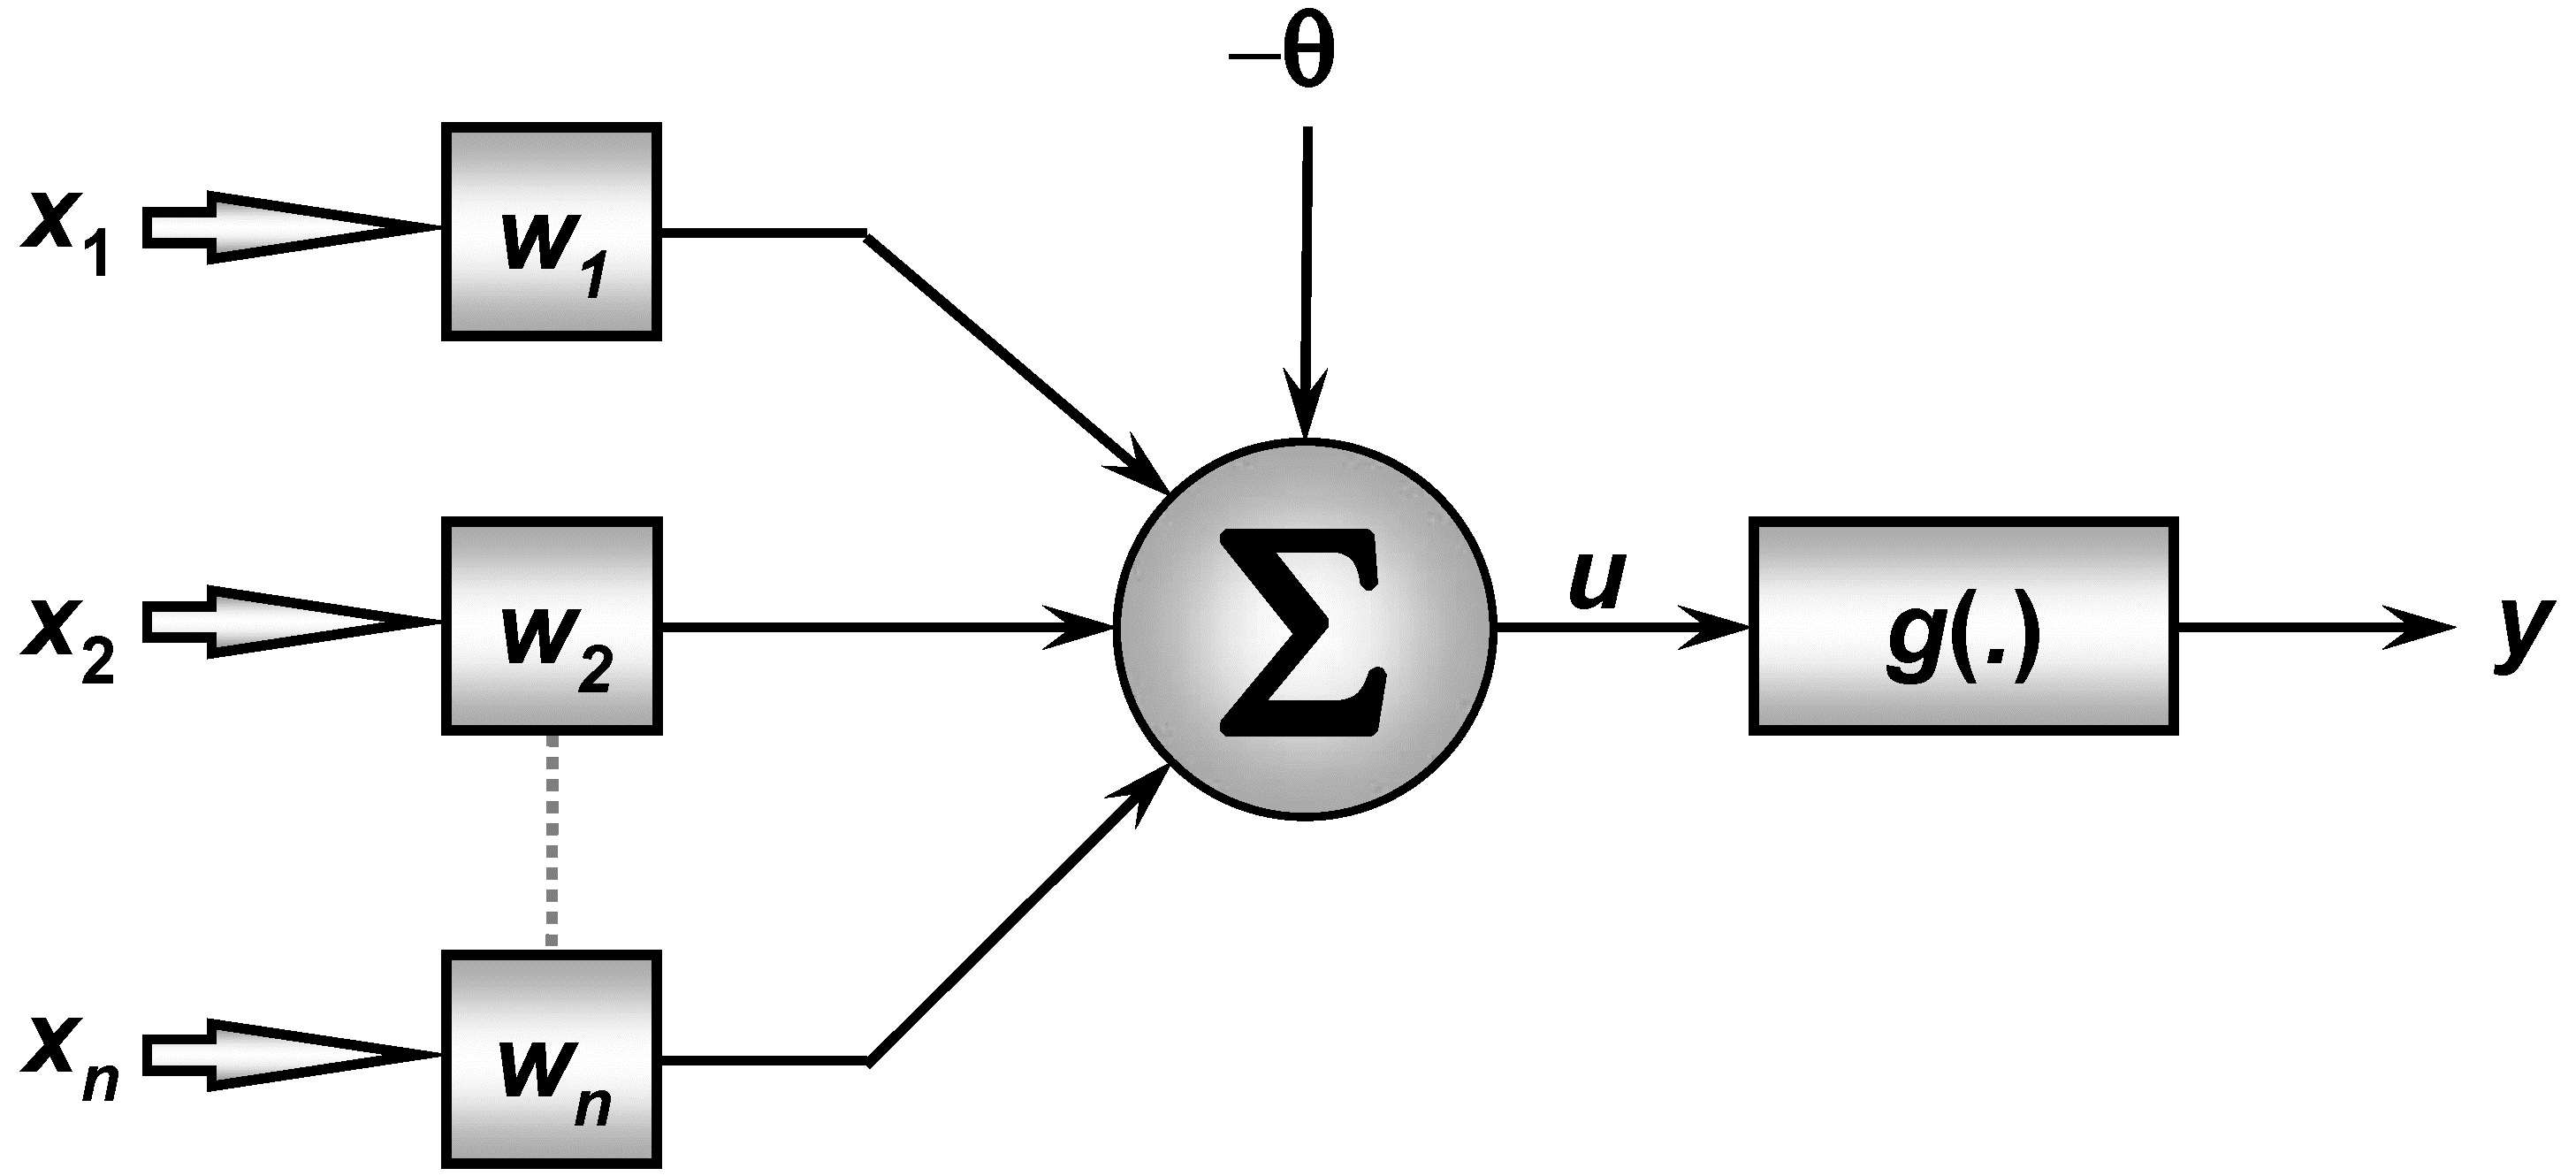
\includegraphics[scale=.2]{imagens/Sadssa.png}
\caption{Exemplo de um neurônio artificial.}
\label{fig:neuronio-artifical}
\end{figure}

Tanto a regressão logística quanto a regressão linear são tipos de perceptrons, que se diferem apensa quanto a função de ativação. Enquanto a regressão logística usa uma sigmóide como \textit{step function}, a regressão linear usa a função identidade \(f(x) = x\). Em uma rede neural uma das funções mais utilizadas é a unidade linear retificada (ReLU), que é uma função não linear.

Quando se usa vários neurônios em paralelo é que se tem uma rede neural. Esses neurônios em paralelo foram a camada oculta. 

Nós podemos tratar o output de cada neurônio como uma variável do input de uma outra camada oculta. Assim, podemos empilhar camadas ocultas e produzir uma rede neural profunda



\section{Trabalhos Relacionados}

Neste capítulo serão apresentados os trabalhos relacionados a esta pesquisa.
Será feito uma contextualização desses trabalhos para depois ser traçado um paralelo entre o que tem sido pesquisado e o que está sendo proposto neste trabalho.
Para fazer essa contextualização foram selecionados 3 dos principais \textit{surveis} que fizeram um grande levantamento do que estava sendo pesquisado na área entre 2010 e 2014, e alguns trabalhos que tem uma relação direta com o tema de pesquisa deste trabalho.

%% 2010 colocar o trabalho de Romero e ventura que é um survei da area de edm

%% 2011
\citealp{Manhaes2011} provaram que é possível identificar alunos em risco de evasão através das primeiras notas semestrais dos alunos ingressantes.
A base de dados utilizada no trabalho foi do sistema acadêmico da instituição e contou com alunos que cursaram Engenharia Civil na UFRJ de 1994 a 2005.
O trabalho consistiu em 3 experimentos, onde foi modificado apenas a forma de treinamento dos algoritmos 10 fold \textit{Cross-validation}, \textit{train/test percentage split (data randomized)} e \textit{supplied test set}, em que 2/3 para treinamento e o restante para teste.
Cada experimento foi submetido a 10 algoritmos utilizados em trabalhos relacionados.
Os experimentos alcançaram acurácia média entre 75\% e 80\%, além disso a predição incorreta de risco de evasão foi considerada como erro grave do classificador.

%% 2014
No trabalho de \citealp{rigo2014aplicaccoes} é apresentado um estudo de fatores envolvidos no fenômeno de evasão escolar e descrevem a utilização de um sistema para MDE e LA durante 18 meses em cursos de graduação na modalidade de Educação a Distância.
Ao todo foram executados 4 experimentos onde foram acompanhados 603, 250, 925 e 713 alunos.
Para cada estudo de caso que trata o trabalho foi utilizado a técnica \textit{RNA Multilayer Perceptron}.
O melhor resultado com relação a predição da evasão foi no experimento 4 onde a melhor média de acertos foi de 83,7\%.

\citealp{Santos2014} propõem identificar precocemente estudantes de graduação EAD em risco de evasão através de técnicas de mineração de dados.
Os autores coletaram dados do AVA e do Sistema de Controle Acadêmico (SCA).
Na base de dados do AVA foram selecionadas as notas intermediárias da disciplina durante o semestre e no SCA foram utilizadas a situação da disciplina, média da disciplina, quantidade de reprovação no período ou semestre e média no período.
Os dados foram submetidos a três algoritmos de classificação baseados em Arvore de Decisão (\textit{SimpleCart}, J48 e \textit{ADTree}), para construção do modelo preditivo.
Os autores relataram que obtiveram um acurácia média de 80\% na predição da evasão, utilizando a primeiras notas semestrais dos estudantes.
Ainda destacam que no AVA chegaram a obter uma acurácia de 98,47\% na predição do desempenho de uma disciplina.

%% 2015
\citealp{detoni2015modelagem} apresentaram uma metodologia para classificar alunos usando apenas a contagem de interação de cursos EAD.
Foram utilizados dados de disciplinas do primeiro e segundo semestre de dois cursos EAD que ocorreram em 2013.
Os autores criaram dois modelos um que utilizou apenas o número absoluto de iterações dos alunos, e outro que foi adicionado atributos derivados do número de iterações.
Foram aplicados quatro modelos de classificação aos dados coletados.
No trabalho foi possível provar que a abordagem de atributos derivados do número de iterações dos alunos obteve resultados superiores a abordagem de trabalhos anteriores.

\citealp{queiroga2015estudo} apresentaram os resultados iniciais de um trabalho voltado para a predição precoce da evasão de alunos em um curso EAD utilizando MDE.
Os autores coletaram os logs das iterações dos alunos de duas turmas de diferentes polos.
Foram realizados 3 experimentos onde o primeiro e segundo experimentos usaram os dados de turmas de diferentes cidade e o terceiro reuniu os 2 conjuntos de dados.
A cada experimento foi aplicado um conjunto de 9 algoritmos de aprendizagem de máquina usando a opção de \textit{Cross-validation}.
A conclusão do trabalho foi de que é viável a predição precoce do risco de evasão através da análise dos logs das 4 primeiras semanas de uma turma.

%% 2016
Em \citealp{hasbun2016extracurricular} foi discutida a importância de atividades extracurriculares para prever o abandono escolar de estudantes de dois cursos de Bacharel em Ciências (Engenharia e Negócios).
Foram coletados dados de 4840 alunos.
Dois modelos foram treinados, uma incluindo todos os dados e outra removendo notas e créditos obrigatórios do valor das atividades.
Ambos os modelos foram treinados e validados usando \textit{Cross-validation}.
A primeira árvore de decisão obteve a melhor precisão (93,94\%).
Para o segundo modelo obteve uma precisão de 79,29\%.
Os autores relataram que embora a previsão de abandono com dados acumulados mostre um melhor desempenho, o segundo modelo ajuda a resolver o problema de disponibilidade de dados dos alunos.
Além disso, a partir da análise dos erros, descobriram que a árvore de decisão treinada com todos os dados foi eficiente na modelagem das expectativas acadêmicas do programa, ocultando fatores pessoais que são mais relevantes para intervenções de prevenção de abandono.
Por isso, os resultados apresentados sugerem que incluir atividades extracurriculares é útil para observar comportamentos específicos que parecem estar relacionados ao fenômeno de desligamento relacionado ao abandono.

\citealp{kantorski2016prediccao} propõem prever a evasão de cursos de graduação presenciais em universidades públicas.
Foram extraídos dados pessoais, acadêmicos, sociais e econômicos de alunos e construídos modelos de predição através de algoritmos de aprendizagem de máquina.
Os autores destacam que a vantagem da proposta foi a otimização dos resultados pela combinação de vários modelos de mineração de dados para gerar uma única predição e isso permite um resultado mais abrangente.
Nos testes alcançaram uma acurácia de 98\% e mais de 70\% de sucesso na predição de alunos que evadiram do curso.

%% 2017

%% 2018
\citealp{lanes2018prediccao} apresentaram um estudo que visa identificar estudantes que apresentam risco de evasão a partir do seu primeiro ano no curso de graduação.
Os experimentos foram realizados com informações extraídas do sistema acadêmico da FURG.
O conjunto de dados contou com 916 registros de 12 cursos de graduação de áreas distintas.
Os dados foram discretizados e categorizados para gerar o \textit{dataset} final.
Foi utilizado a ferramenta Weka e aplicado o algoritmo J48 para processar o \textit{dataset} e obter a arvore de decisão.
Os resultados mostram que os potenciais alunos em risco de evadir podem ser identificados com acurácia de 90,7\% usando o algoritmo J48.

% Quais as características destes artigos, quais os pontos que teu trabalho é diferente deles. Precisas dizer algo como: Nos trabalhos apresentados eles focam em tal domínio, ou apontam tal técnica, e no nosso, focamos de outra maneira, outra técnica, outro domínio... 


% criar uma seção de conclusão do capítulo
% deve falar da evasão, mde, e trabalhos relacionados

\section{Conclusão do capítulo}

Foram selecionados trabalhos diretamente relacionados a predição da evasão escolar em sistemas acadêmicos, mas também foram analisados parcialmente trabalho não relacionados diretamente com o objetivo principal da pesquisa. Outro trabalhos que usaram dados retirados de AVA como \citet{Braz2019}, \citet{Burlamaqui2017}, \citet{detoni2015modelagem}, \citet{Fernandes2017}, \citet{queiroga2015estudo}, \citet{Ramos2018}, \citet{Santos2014} e \citet{Silva2015}. Ou trabalhos que não foram com alunos do ensino superior tais como \citet{Bezerra2016}, \citet{Calixto2017} e \citet{Sales2019}, dentre outros.

A principal diferença deste trabalho é a aplicação de técnicas de visualização e MDE em cima de dados reais de alunos do curso presencial de Ciência da Computação da UFPel.
% Além disso utilizamos \textit{train/test percentage split (data randomized)}, para poder aplicar técnicas de \textit{oversampling} e \textit{undersampling} na base de treinamento.
Outro ponto a ser levado em consideração é que foi utilizado apenas um curso para tentar não generalizar e evitar problemas como o paradoxo de Simpson.
Também foi feito uma caracterização da evasão em cima de dados de 20 anos do curso.
Por fim, diferentemente dos outros trabalhos foram utilizados dados apenas dos 3 primeiros semestres do curso.

\chapter{Metodologia}
\label{cap:metodologia}

No decorrer desta dissertação foram alcançados resultados iniciais que serviram para definir a metodologia utilizada neste trabalho, e também foram publicados em eventos como LACLO 2020 e EMPOS 2020.

Neste capítulo será apresentada a metodologia que norteou o desenvolvimento desta pesquisa.
A metodologia CRISP-DM que tem como principal objetivo fornecer uma direção para conduzir o processo de KDD \cite{goldschmidt2015data}.
A figura \ref{fig:fases-metodologia-crips-dm} apresenta o ciclo de vida dividido em 6 fases da metodologia CRISP-DM.
A seguir será apresentado uma breve descrição das seis fases da metodologia:

\begin{figure}[htbp]
\centering 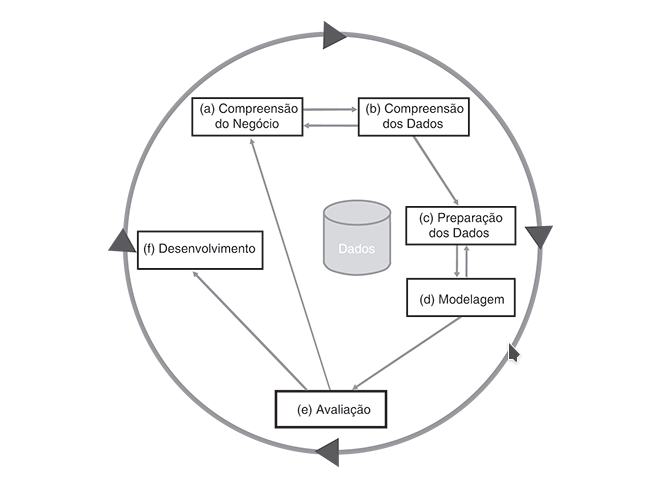
\includegraphics[scale=.7]{imagens/fase-metodologia-crisp-dm.png}
\caption{Fases do modelo de referência CRISP-DM. Adapitado de Shearer (2000). Fonte: \cite{goldschmidt2015data}.}
\label{fig:fases-metodologia-crips-dm}
\end{figure}

\begin{enumerate}
\item \textbf{Compreensão do negócio:} Esta é a fase onde se deve identificar o problema a ser resolvido. Esta fase compreende também uma descrição do \textit{background}, dos objetivos e também dos critérios de sucesso \cite{Melo2007}. Esta fase não será descrita no presente capítulo, pois já feito no Capítulo \ref{cap:referencial-teorico}.
\item \textbf{Compreensão dos dados:} É a fase responsável por fazer a coleta dos dados e a análise exploratória de dados (AED). Esta fase tem que dizer como os dados foram adquiridos, qual o seu formato, qual foi a quantidade de dados, descrever cada atributo selecionado, fazer visualizações dos dados e além disso qualquer informação pertinente aos dados.
\item \textbf{Preparação dos dados:} Compreende as atividades de pré-processamento dos dados para a próxima fase. Normalmente se faz a seleção, limpeza, formatação dos dados, e ainda gera-se novos atributos derivados dos atributos existentes.
\item \textbf{Modelagem:} Corresponde a fase de aplicação dos algoritmos de mineração de dados selecionados sobre os dados preparados. É a etapa de mineração de dados do processo de KDD \cite{goldschmidt2015data}. Nessa fase é criado um modelo para testar a sua qualidade e validade. É comum usar a taxa de erro como medida de qualidade do modelo em aprendizado supervisionado \cite{Melo2007}.
\item \textbf{Avaliação:} Consiste em avaliar o modelo gerado, examinando os passos seguidos e validando se realmente foram alcançados os objetivos elencados na fase de compreensão do negocio \cite{Melo2007}. A partir da avaliação é possível propor revisões das fases anteriores e redefinir os próximos passos \cite{goldschmidt2015data}.
\item \textbf{Desenvolvimento:} É a fase onde se faz o planejamento e acompanhamento a serem realizadas com o modelo gerado pelas fases anteriores \cite{goldschmidt2015data}. Esta fase não faz parte do escopo deste trabalho.
\end{enumerate}

Este capítulo será dividido conforme as etapas da metodologia CRISP-DM.

\section{Compreensão dos dados}
\label{sec:compreensao-dados}

Aqui, você deverá coletar, descrever — usando estatísticas — , explorar e verificar a qualidade do seu dado.

Nesta sessão será apresentada como foi feito a coleta, descrição e a análise exploratória dos dados. 
Por serem tarefas manuais foi uma das etapas que demandaram mais tempo deste trabalho.

As ferramentas desta fase foram utilizadas em um sistema Debian Buster.
Nesta fase foram utilizadas as seguintes ferramentas:

\begin{itemize}
    \item Pgadmin3: foi utilizado para as consultas SQL;
    \item Mozzila Firefox: navegador utilizado para acessar a ferramenta de modelagem;
    \item Google Colab: ferramenta que cria um ambiente virtual que disponbiliza diversos recurso em Python;
    \item Python: linguagem de programação;
    \item Pandas: biblioteca do Python utilizada para manipulação de dados;
    \item seabor: biblioteca do Python utilizada para gerar os gráficos; 
\end{itemize}

\subsection{Coleta dos dados}
\label{subsec:coleta-dos-dados}

Neste trabalho foram utilizados os dados de alunos do curso de Ciência da Computação registrados no Cobalto, que é o sistema gestão da UFPel.
O Cobalto é um sistema integrado de gestão que faz a gestão acadêmica da universidade.
Este sistema possui dados históricos de alunos, importados do sistema anterior da IES, denominado GOL.

Os dados extraídos do sistema correspondem aos alunos do curso de Ciência da Computação que ingressaram entre os anos 2000 e 2020.
Os dados sociais e acadêmicos dos alunos foram extraídos através de consultas diretas a base de dados do sistema acadêmico.
Vale destacar que esses dados foram anonimizados, ou seja, foi utilizado um código de identificação fictício para cada aluno.

A Tabela~\ref{tab-totais} apresenta o número total de matrículas e de alunos para a situação final ou atual.
Nesta seção o termo matrícula será usado para identificar a matrícula em uma disciplina, ou seja quando quiser falar que um aluno se matriculou em 6 disciplinas será falado que o aluno tem 6 matriculas.
A situação ``Cursando'' representa todos os alunos que ainda estão dentro do período de integralização curricular e não saíram do curso.
Já a situação ``Retido'' são todos os alunos que já passaram do período de integralização curricular e não tem saída. As situações ``Formado'' e ``Evadido'' são alunos que já tem uma saída registrada.

\begin{table}[htbp]
% \footnotesize\addtolength{\tabcolsep}{-3pt}
\begin{center}
\caption{Resumo dos totais de dados coletados}\label{tab-totais}
\begin{tabular}{p{2cm}|p{2cm}|p{2cm}|p{2cm}|p{2cm}|p{2cm}}
\hline
\multicolumn{1}{c|}{\multirow{Matriculas}} & \multicolumn{5}{c}{Alunos} \\ \cline{2-6} \multicolumn{1}{c|}{} & \multicolumn{1}{l|}{Total} & \multicolumn{1}{l|}{Cursando} & \multicolumn{1}{l|}{Evadido} & \multicolumn{1}{l|}{Formado} & Retido  \\ \hline
% 21000       & 1516      & 287      & 785     & 328     & 116    \\ % antes de 6 de novembro de 2020
21105 & 1514 & 286 & 786 & 330 & 112 \\
\hline
\end{tabular}
\end{center}
\end{table}

Nesta pesquisa foram utilizados os dados dos três primeiros semestres de alunos do curso de Ciência da Computação.
A ideia de utilizar os dados dos três primeiros semestres é que quanto mais cedo identificar o aluno propenso a evadir maior é a chance de fazer um planejamento de ações para poder modificar essa situação.
Trabalhos como o de \citealp{lanes2018prediccao} tiveram exito usando esse mesmo tipo de abordagem.

\subsection{Descrição dos dados}
\label{subsec:descricao-dos-dados}

Nesta seção serão apresentados os atributos retirados da base de dados. Para chegar no conjunto final de atributos foram feitos diversas tentativas. Abaixo segue a lista de todos os atributos utilizados neste trabalho e sua respectiva descrição:

\begin{itemize}
\item cod\_aluno: Identificador do aluno. 
\item ano\_ingresso e semestre\_ingresso: Ano e semestre que o aluno ingressou no curso. 
\item ano\_saida e semestre\_saida: Ano e semestre que o aluno saiu do curso. 
\item aluno\_situacao: Situação final do aluno no curso.
\item nota\_final: Nota final do aluno em uma disciplina. 
\item ano\_disciplina e semestre\_disciplina: Ano e semestre que o aluno cursou a disciplina. 
\item disciplina\_situacao: Situação do aluno na disciplina. 
\item genero: Gênero do aluno.
\item dt\_nascimento: Data de nascimento do aluno. 
\item dt\_ingresso: Data de ingresso no curso. 
\item etnia: Etnia do aluno. 
\item estado\_civil: Estado civil do aluno. 
\item tipo\_ingresso: Forma de ingresso do aluno.
\item cota: Cota de ingresso do aluno. 
\item flg\_escola\_publica: Aluno veio de escola pública.  
\item flg\_curso\_superior: Aluno concluiu ensino superior anterior.  
\item flg\_benefício: Aluno recebeu auxílio.  
\item naturalidade: Cidade natal do aluno.  
\item flg\_pri\_sem: Indica que o aluno cursou a disciplina no primeiro semestre.
\item flg\_seg\_sem: Indica que o aluno cursou a disciplina no segundo semestre.
\item flg\_ter\_sem: Indica que o aluno cursou a disciplina no terceiro semestre. 
\item nr\_dis\_pri\_sem\_cur: Número de disciplinas do primeiro semestre do curriculo do aluno.
\item nr\_dis\_seg\_sem\_cur: Número de disciplinas do primeiro semestre do curriculo do aluno.
\item nr\_dis\_ter\_sem\_cur: Número de disciplinas do primeiro semestre do curriculo do aluno.
\item tempo\_total\_curso: Número de semestres que o aluno cursou ou está cursando no curso. 
\end{itemize}

Abaixo será a apresentado os dados estatísticos de cada atributos. O atributo cod\_aluno será desconsiderado, pois é apenas um identificador.

\subsubsection{ano\_ingresso e semestre\_ingresso}
\label{subsubsec:ano-semestre-ingresso}

Os atributos ano\_ingresso e semestre\_ingresso correspondem, respectivamente, ao ano e semestre de ingresso do aluno no curso. A figura \ref{fig:nr-alunos-pelo-ano-semestre-ingresso} mostra o número de alunos que ingressaram pelo ano e semestre de ingresso. O período que teve o maior número de ingressantes foi de 2009/1, onde ingressaram 60 alunos. O período com o menor número de ingressantes foi 2002/1, mas é preciso investigar este caso pois pode ser apenas uma sujeira na base de dados.

O atributo ano\_ingresso pode assumir o valor entre 2000 e 2020, para o conjunto de dados extraído da base. Já o semestre\_ingresso pode assumir os valores 1 ou 2, que representam respectivamente o primeiro e segundo semestre do ano.

\begin{figure}[htbp]
\centering 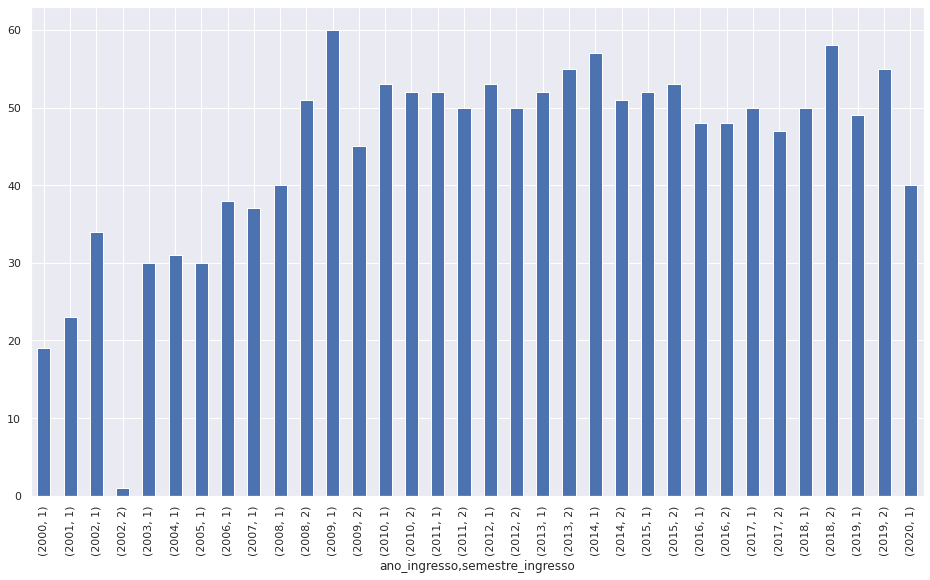
\includegraphics[scale=.41]{imagens/nr-alunos-pelo-ano-semestre-ingresso.png}
\caption{Número de alunos pelo ano e semestre de ingresso no curso.}
\label{fig:nr-alunos-pelo-ano-semestre-ingresso}
\end{figure}

\subsubsection{ano\_saida e semestre\_saida}
\label{subsubsec:ano-semestre-saida}

Estes atributos são o ano e semestre que o aluno perdeu o vinculo com a UFPel.
O período com o maior número de saídas foi 2013/1 com mais de 70 alunos.
Além disso eles podem assumir os mesmos valores que o ano\_ingresso e semestre\_ingresso.
Estes atributos possuem 408 registros com valores nulos, estes são alunos que ainda estão no curso e por isso não tem um período de saída.

\begin{figure}[htbp]
\centering 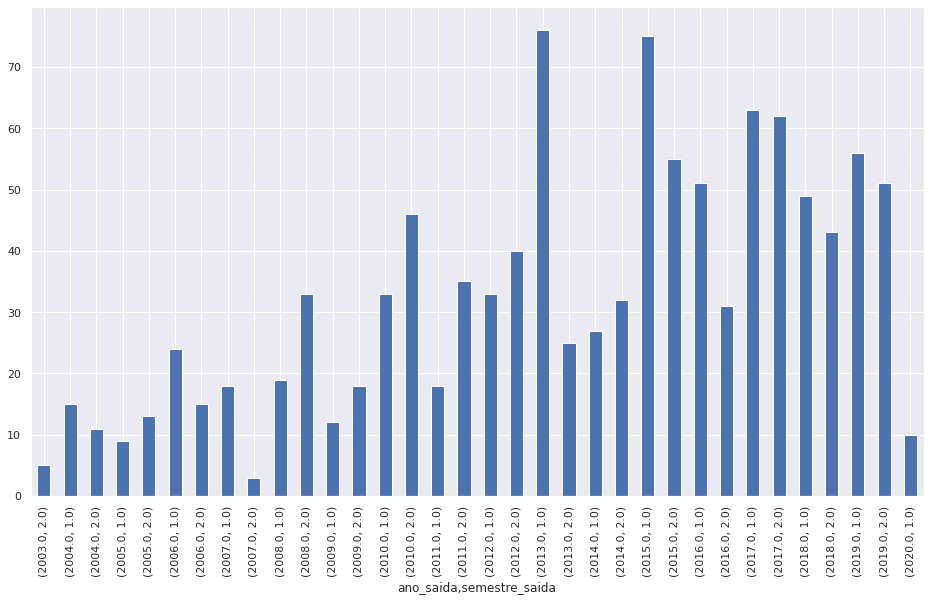
\includegraphics[scale=.41]{imagens/nr-alunos-pelo-ano-semestre-saida.png}
\caption{Número de alunos pelo ano e semestre de ingresso no curso.}
\label{fig:nr-alunos-pelo-ano-semestre-saida}
\end{figure}

A figura \ref{fig:nr-alunos-pelo-ano-semestre-saida} mostra o ano e semestre que o aluno perdeu o vínculo com a instituição. O período com o maior número de saídas foi 2013/2. Estas saídas podem envolver qualquer situação listada na seção \ref{subsubsec:aluno-situacao}.

\subsubsection{aluno\_situacao}
\label{subsubsec:aluno-situacao}

Este atributo é a situação do aluno no curso e serve para definir a situação final ou atual do aluno no Curso. A partir deste atributo será criado um novo atributo ``evadiu''. Neste trabalho o atributo ``evadiu'' será a variável preditora (\textit{predicted variable}) que identifica se o aluno evadiu ou não do curso.
Para esta variável os modelos tem que prever se o aluno consegui concluir o curso (N) ou não consegui (S).

A tabela \ref{tab:situacoes-alunos} mostra os tipos de situações encontradas no conjunto de dados da Ciência da Computação e o total de alunos em sua respectiva situação.
A maioria das ocorrência são de alunos em situação de ``Abandono'' que representa mais de 30\% de alunos de toda a base de dados, enquanto que alunos na situação ``Formado'' 21,80\% do total. 
Para o curso de Ciência da Computação foram encontradas 15 situações diferentes para o conjunto de dados.

Na seção \ref{subsubsec:ano-semestre-saida} foram encontrados 408 alunos sem o ano e semestre de saída, mas o total de ``Aluno com vínculo'' é de 398 alunos.
Isso acontece pois existem situações que são consideras como saída do aluno e outras não.
No caso do curso de Ciência da Computação, alunos na situação de ``Aluno com vínculo'' e ``Trancamento'' são situações que não são considerada como situações de saída do aluno. Todas as outras situações são consideradas como saída do aluno.

\begin{table}[htbp]
\begin{center}
\caption{Tipos de situações de alunos.}
\label{tab:situacoes-alunos}
\begin{tabular}{p{10cm}|p{5cm}}
\hline
Situação                                & Nr. alunos\\ \hline
Abandono                                & 477\\
Aluno com vínculo                       & 398\\
Cancelamento                            & 202\\
Desligado                               &   1\\
Desligado Lei nº 12.711 de 29/08/2012   &   2\\
Desligado Res.03/05                     &   4\\
Falecido                                &   1\\
Fim Mobilidade                          &   1\\
Fim período                             &   2\\
Formado                                 & 330\\
Jubilado                                &   3\\
Matrícula não confirmada                &  11\\
Reopção                                 &  50\\
Trancamento                             &  10\\
Transferido                             &  22\\
\hline
\end{tabular}
\end{center}
\end{table}

\subsubsection{nota\_final}

Este atributo é a nota que o aluno obteve na disciplina.
Foram coletado 21.105 matriculas de alunos em disciplinas, dessas 18.500 tem valores registrado e 12,34\% tem valores nulo.


\begin{table}[htbp]
\begin{center}
\caption{Dados estatísticos da nota final do aluno}
\label{tab:nota-final}
\begin{tabular}{p{8cm}|p{7cm}}
\hline
Dado estatístico & Valor    \\ \hline
count   & 18500    \\
mean    & 5.44     \\
std     & 3.36     \\
min     & 0.00     \\
25\%    & 2.10     \\
50\%    & 7.00     \\
75\%    & 8.20     \\
max     & 10.00    \\ \hline
\end{tabular}
\end{center}
\end{table}

A nota final é um atributo numérico e pode assumir valores de 0 a 10.
A tabela \ref{tab:nota-final} apresenta os dados esteatíticos do atributo nota\_final. 
A média geral das notas foi de 5,44 com o desvio padrão de 3,36.

\subsubsection{ano\_disciplina e semestre\_disciplina}

Estes atributos representam o ano e semestre que o aluno cursou a disciplina e serão usado para definir em qual semestre do curso o aluno fez a disciplina.
O atributo ano pode assumir qualquer valor entre 2000 e 2020, e o atributo semestre pode ser 1 para primeiro semestre e 2 para segundo semestre.

\begin{figure}[htbp]
\centering 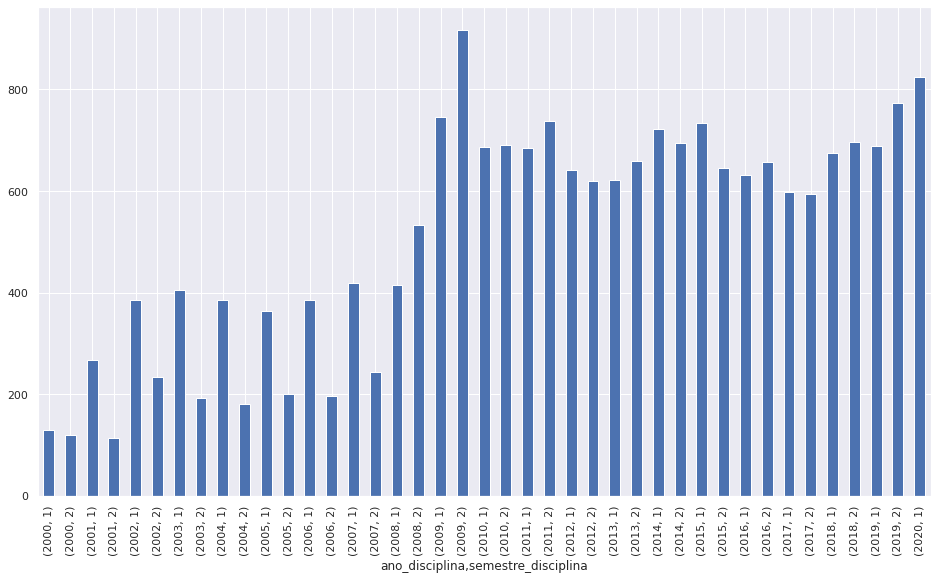
\includegraphics[scale=.41]{imagens/ano-semestre-disciplina.png}
\caption{Número de disciplinas cursadas pelo ano e semestre.}
\label{fig:nr-disciplinas-cursadas-ano-semestre}
\end{figure}

\subsubsection{disciplina\_situacao}

Atributo usado para registrar a situação da disciplina em um determinado semestre.
A maior frequência é da situação Aprovados com 11.803 matriculas nesta situação.

Este atributo junto com o ano e semestre da disciplina vai ser usado para fazer a contagem de quantas disciplinas o aluno aprovou em um determinado semestre. 

Algumas situações serão removidas na etapa de limpeza dos dados.
Uma delas é a situação ``DSP'', pois é uma disciplina que o aluno não curso neste vinculo dele.

Outras situações terão que ser analisadas melhor, para veneficiar o que significam. Este é o caso de situação como ``MAT'', ``FRC'', ``UPD'' e ``N/I''.

\begin{table}[htbp]
\begin{center}
\caption{Total de matriculas por situação}
\label{tab:disciplina-situacao}
\begin{tabular}{p{4.5cm}|p{3.5cm}|p{6.5cm}} \hline
Situação da matricula & Nr. de matriculas & Descrição \\ \hline
APR  & 11803 & Aprovados \\
REPR &  3532 & Reprovados \\
INFR &  3080 & Infrequentes \\
MAT  &  1045 & Matriculados \\
DSP  &   856 & Dispensados \\
TRC  &   634 & Trancados \\
CANC &   108 & Cancelados \\
FRQ  &    39 & Frequentes \\
UPD  &     5 & Aprovados usados para dispensa \\
N/I  &     3 & Não informado \\ \hline
\end{tabular}
\end{center}
\end{table}

A tabela \ref{tab:disciplina-situacao} lista todas as situações encontradas para o curso de Ciência da Computação.
Ao todo são 10 situações diferentes para as matriculas encontradas no curso.

\subsubsection{genero}

Representa o gênero do aluno e pode assumir dois valores ``M'' para masculino e ``F'' para feminino.
No curso de Ciência da computação a maior frequência é de homens, com 86,12\% de um total de 1514 alunos.

\begin{table}[htbp]
\begin{center}
\caption{Total de alunos pelo gênero}
\label{tab:total-aluno-genero}
\begin{tabular}{p{7.5cm}|p{7cm}} \hline
Atributo & Nr. total \\ \hline
M  & 1304 \\
F  &  210 \\ \hline
\end{tabular}
\end{center}
\end{table}

A tabela \ref{tab:total-aluno-genero} mostra os quantitativos do gênero masculino e feminino. 

\subsubsection{dt\_ingresso e dt\_nascimento}

Os atributos dt\_ingresso e dt\_nascimento são a data de ingresso do aluno no curso e data de nascimento do aluno respectivamente. Estes atributos vão gerar um novo atributo que vai representar a idade do aluno quando ingressou no curso.

Dos 1514 alunos 36 não possuem data de nascimento registrada no sistema, ou seja, 2,38\% do conjunto de dados total.

\begin{figure}[htbp]
\centering 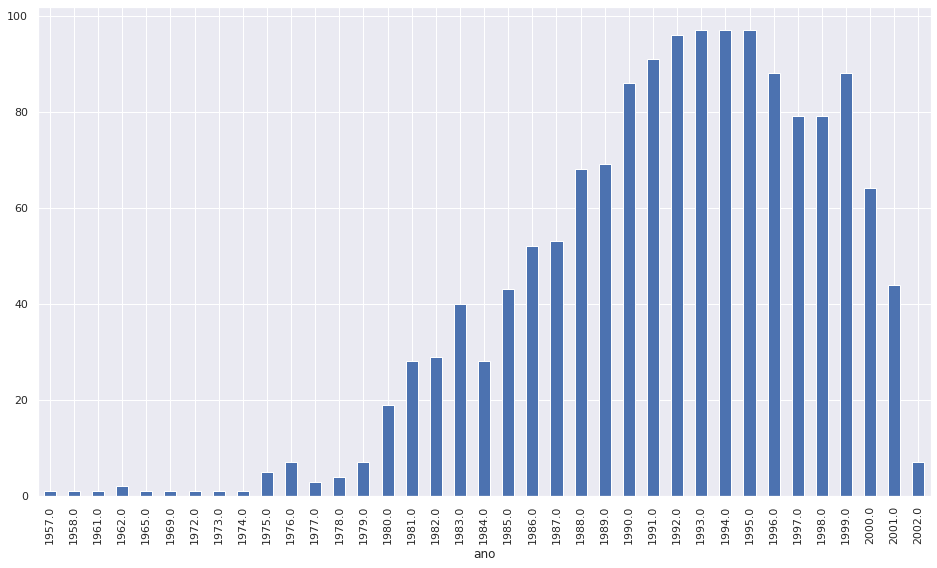
\includegraphics[scale=.48]{imagens/ano-de-nascimento.png}
\caption{Número de alunos pelo ano de nascimento.}
\label{fig:nr-alunos-pelo-ano-nascimento}
\end{figure}

O figura \ref{fig:nr-alunos-pelo-ano-nascimento} mostra a contagem do número total de alunos e seu respectivo ano de nascimento. Alunos que nasceram entre os anos de 1993 e 1995 foram encontrados com maior frequência no curso.

Um dado que chama atenção são é o número de alunos que nasceram em 2002 ser baixo, visto que estes alunos estariam completando 18 anos em 2020. Em análise posterior será necessário verificar com que idade a maior parte dos alunos vem ingressando no curso.

\subsubsection{etnia}

Está atributo é etnia declarada pelo aluno.
Faltam informações de 457 alunos que representa 30,18\% de 1514 alunos.

\begin{table}[htbp]
\begin{center}
\caption{Total de alunos por etnia}
\label{tab:total-etnia}
\begin{tabular}{p{8.5cm}|p{6cm}} \hline
Valor & Nr. total \\ \hline
BRANCA & 749 \\
NÃO QUERO DECLARAR & 167 \\
PARDA &  73 \\
PRETA &  64 \\
AMARELA & 4 \\ \hline
\end{tabular}
\end{center}
\end{table}

A tabela \ref{tab:total-etnia} apresenta o número total de alunos pela sua respectiva etnia.
A maior ocorrência é de alunos de etnia branca 749 dos 1.514 alunos.
Um valor que chama a atenção é de alunos que não querem declarar.

\subsubsection{estado\_civil}

Este atributo é o estado civil do aluno quando ingressou no curso.
Faltam as informações de 495 alunos que representa 32,69\% do total de alunos.

\begin{table}[htbp]
\begin{center}
\caption{Total de alunos pelo estado civil}
\label{tab:total-alunos-estado-civil}
\begin{tabular}{p{8.5cm}|p{6cm}} \hline
Valor      & Nr. total \\ \hline
SOLTEIRO   & 980 \\
CASADO     &  28 \\
OUTROS     &   8 \\
DIVORCIADO &   2 \\
VIUVO      &   1 \\ \hline
\end{tabular}
\end{center}
\end{table}

A tabela \ref{tab:total-alunos-estado-civil} mostra o número total de alunos e seu respectivo estado civil.
A maior ocorrência é de alunos no estado civil ``SOLTEIRO'' com 980 de 1.514 alunos.

\subsubsection{tipo\_ingresso}

O atributo tipo\_ingresso representa a forma de ingresso do aluno no curso.
Este atributo sofreu uma mudança bem significativa depois de 2007, devido a UFPel ter adotado como forma de ingresso o ``SiSU/ENEM''. Isso fez com que alunos que tem a forma de ingresso ``Vestibular'' fossem extintos e é preciso avaliar melhor a utilização desse atributo.

\begin{table}[htbp]
\begin{center}
\caption{Número total de alunos pela forma de ingresso}
\label{tab:total-aluno-tipo-ingresso}
\begin{tabular}{p{8.5cm}|p{6.5cm}} \hline
Valor                                   & Nr. total \\ \hline
SiSU/ENEM                               & 903 \\
Vestibular                              & 383 \\
PAVE                                    & 118 \\
Transferência                           & 50 \\
Reopção                                 & 36 \\
Reingresso                              & 8 \\
Portador de Diploma de Curso Superior   & 8 \\
Decisão Judicial                        & 3 \\
Transferência Compulsória               & 2 \\
Atividades Isoladas                     & 1 \\
Mobilidade Acadêmica                    & 1 \\
Regime Especial                         & 1 \\ \hline
\end{tabular}
\end{center}
\end{table}

A tabela \ref{tab:total-aluno-tipo-ingresso} mostra o número total de alunos e sua respectiva forma de ingresso no curso de Ciência da computação.
A maior ocorrência é de ``SiSU/ENEM'' com 903 alunos, que representa 59,64\% do total de alunos.


\subsubsection{cota}

Este atributo identifica por qual cota o aluno ingressou.
De 629 alunos a cota de ampla concorrência representa aproximadamente 50\% do total das formas de ingresso.
Pela forma de ingresso da universidade nem sempre sido feita por cotas este atributo tem muitos dados faltando e não será possível utiliza-lo.

\begin{table}[htbp]
\begin{center}
\caption{Número total de alunos pela cota de ingresso.}
\label{tab:total-alunos-cota-ingresso}
\begin{tabular}{p{8.5cm}|p{6cm}} \hline
Valor & Nr. total \\ \hline
AC    & 318 \\
L05   & 125 \\
L01   & 95 \\
L06   & 45 \\
L02   & 44 \\
L13   & 2 \\ \hline
\end{tabular}
\end{center}
\end{table}

\subsubsection{flg\_escola\_publica}

Este atributo indica se o aluno veio de escola pública ou não.
Existem sujeiras na base que precisarão ser identificas, e corrigidas ou eliminadas.

\begin{table}[htbp]
\begin{center}
\caption{Número de alunos que vem ou não de escola pública}
\label{tab:total-aluno-escolca-publica}
\begin{tabular}{p{8.5cm}|p{6cm}} \hline
Valor & Nr. total \\ \hline
S     & 982 \\
N     & 391 \\
P     &  23 \\
V     &  22 \\ \hline
\end{tabular}
\end{center}
\end{table}

\subsubsection{flg\_curso\_superior}

Este atributo indica se o aluno cursou algum curso superior antes do curso atual. Caso o aluno tenha curso supeiro anterior o valor desse atributo é 'S' acaso contrário é 'N'.

Aproximadamente 98\% dos alunos da Ciência da Computação não possuem curso superior anterior.

\begin{table}[htbp]
\begin{center}
\caption{Total de aluno que possui ou não curso superior anterior}
\label{tab:total-aluno-curso-superior-anterior}
\begin{tabular}{p{8.5cm}|p{6cm}} \hline
Valor & Nr. total \\ \hline
N     & 1491 \\
S     &   23 \\ \hline
\end{tabular}
\end{center}
\end{table}

\subsubsection{flg\_beneficio}

Este atributo informa se o aluno possui ou não benefício e não apresenta qualquer tipo de erro nesta analise. Pode assumir o valor "S" se possui o benefício ou "N" caso contrário.

Mais de de 77\% dos alunos não possui benefício.
O problema deste atributo é que o número de registro de benefícios ficou mais relevante a partir de 2004 com 206 registros de benefícios.

\begin{table}[htbp]
\begin{center}
\caption{Total de alunos que possui ou não benefício}
\label{tab:total-aluno-beneficio}
\begin{tabular}{p{8.5cm}|p{6cm}} \hline
Valor & Nr. total \\ \hline
N     & 1167 \\
S     &  347 \\ \hline
\end{tabular}
\end{center}
\end{table}

\subsubsection{naturalidade}

Este atributo foi adaptado para 6 categorias:

\begin{itemize}
\item PELOTAS - Alunos que nasceram na cidade de Pelotas;
\item MICROPELOTAS - Alunos que nasceram na Microregião de Pelotas;
\item MESOPELOTAS - Alunos que nasceram na Mesoregião de Pelotas;
\item ESTADO - Alunos que nasceram no estado do Rio Grande do Sul;
\item PAIS - Alunos que nasceram fora do estado do Rio Grande do Sul;
\item ESTRANGEIRO - Alunos que nasceram em qualquer cidade fora do Brasil.
\end{itemize}

Neste atributo faltam informações de 335 alunos, que representa 22,13\% do total de alunos.

\begin{table}[htbp]
\begin{center}
\caption{Total de alunos pela naturalidade.}
\label{tab:total-alunos-naturalidade}
\begin{tabular}{p{8.5cm}|p{6cm}} \hline
Valor & Nr. total \\ \hline
PELOTAS         & 562 \\
MICROPELOTAS    & 105 \\
MESOPELOTAS     & 56  \\
ESTADO          & 252 \\
PAIS            & 204 \\ \hline
\end{tabular}
\end{center}
\end{table}

\subsubsection{flg\_pri\_sem, flg\_seg\_sem, flg\_ter\_sem, nr\_dis\_pri\_sem\_cur, nr\_dis\_seg\_sem\_cur e nr\_dis\_ter\_sem\_cur}

Este atributos vão servir para criar o coeficiente de ralação, que vai ser o número de disciplinas aprovadas no semestre dividido pelo número de disciplinas no currículo do curso no respectivo semestre.

\subsection{Análise exploratória dos dados}

% Referenciar essa parte palavras de 3 estudos Castro et al. 2007, Baker 2009; Dekker et al. 2009
% Estes estudos são importantes, porque mostram as dificuldades de fazer a coleta de dados que ainda é um trabalho manual, e que esses dados precisam passar por um processo, pois não são diretamente tratados pelos algoritmos de aprendizagem.
% 
% Castro F. et al. (2007) “Applying Data Mining Techniques to e-Learning Problems, Studies in Computational Intelligence (SCI).” 62, 183 - 221 (2007) Springer-Verlag Berlin Heidelberg.
% Baker, R. and Yacef K. (2009) “The State of Educational Data Mining in 2009: A Review and Future Visions.” Pages 3-17. JEDM -Journal of Educational Data Mining, 2009, Volume 1, Issue 1, October 2009
% Dekker G., Pechenizkiy M. and Vleeshouwers J. (2009) “Predicting Students Drop Out: A Case Study”. In Proceedings of the International Conference on Educational Data Mining, Cordoba, Spain, T. BARNES, M. DESMARAIS, C. ROMERO and S. VENTURA Eds., Pages 41-50.
% Os principais pontos são: i) transformação dos dados (os dados colhidos nem sempre são diretamente tratados pelos algoritmos de mineração); ii) identificar os atributos mais relevantes; iii) identificar os algoritmos mais adequados; iv) aplicar os algoritmos para identificar outros grupos de estudantes.

% NESTA PARTE SERÃO FEITAS ALTERAÇÕES NOS GRAFICOS E SERÁ MOSTRADO MAIS TABELAS.
% GRAFICOS A SEREM MOSTRADOS:
% - Gráficos mostrando os alunos por idade, bem como a tabela mostrando os percentuais; Obs.: os graficos e tabelas estão no arquivo ciencia_computacao_aed

Neste trabalho foi feito uma AED para entender a natureza dos dados sem fazer suposições e tentar tirar alguns \textit{insights}.
A AED é uma técnica realizada após a etapa de pré-processamento de dados e coleta de dados.

Para fazer algumas análises foi criado um campo chamado ``Situação categoria'', que agrupa as situações dos alunos apresentada na seção \ref{subsubsec:aluno-situacao} em 4 classes ``Cursando'', ``Retido'', ``Formado'' e ``Evadido''.
A tabela \ref{tab:situacoes-alunos-classes} mostra a relação das situações dos alunos com as novas classes. As classes ``Cursando'' e ``Retido'' foram determinadas pela seguinte regra: alunos que estavam nas situações ``Aluno com vínculo'' ou ``Trancado'', e além disso estava a mais de 8 semestres no curso foram considerados como ``Retido'' caso contrário foram considerados como ``Cursando''.

\begin{table}[htbp]
\begin{center}
\caption{Relação de situações e novas classes.}
\label{tab:situacoes-alunos-classes}
\begin{tabular}{p{10cm}|p{5cm}} \hline
Situação                                & Categorias         \\ \hline
Abandono                                & Evadido            \\
Aluno com vínculo                       & Cursando ou Retido \\
Cancelamento                            & Evadido            \\
Desligado                               & Evadido            \\
Desligado Lei nº 12.711 de 29/08/2012   & Evadido            \\
Desligado Res.03/05                     & Evadido            \\
Falecido                                & Evadido            \\
Fim Mobilidade                          & Evadido            \\
Fim período                             & Evadido            \\
Formado                                 & Formado            \\
Jubilado                                & Evadido            \\
Matrícula não confirmada                & Evadido            \\
Reopção                                 & Evadido            \\
Trancamento                             & Cursando ou Retido \\
Transferido                             & Evadido            \\ \hline
\end{tabular}
\end{center}
\end{table}

\subsubsection{Idade}

A idade do aluno foi formada usando o ano de nascimento do aluno menos o ano de ingresso do aluno no curso, então foi considerada a idade que o aluno tinha quando ingressou no curso.
Por existirem alunos com data de nascimento nulo foram considerados apenas 1.475 alunos ao invés dos 1.514 coletados da base de dados.

A figura \ref{fig:histograma-idade} é um histograma, que mostra a densidade de alunos por idade.
A partir do gráfico é possível verificar que a idade dos alunos esta concentrada no inicio, ou seja, a maior parte dos alunos são jovens com idade entre 16 e 21 anos. Outro ponto importante é que o gráfico não segue uma distribuição normal, pois a concentração de dados não está no meio do gráfico.


\begin{figure}[htbp]
\centering 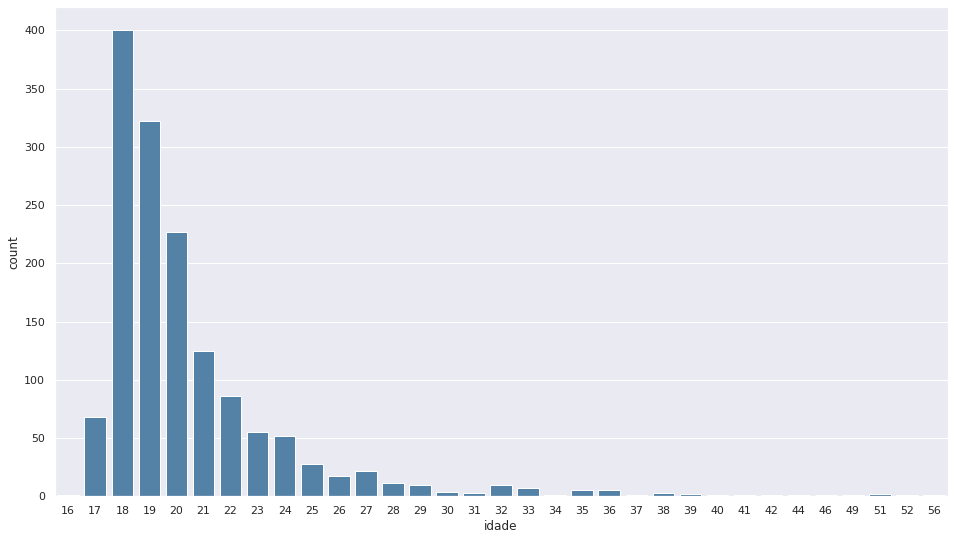
\includegraphics[scale=.45]{imagens/histograma-idade.png}
\caption{Número de alunos por idade de ingresso no curso.}
\label{fig:histograma-idade}
\end{figure}

\subsubsection{Idade x Situação}

Nesta seção será cruzado a idade dos alunos com a situação final deles.
A figura \ref{fig:media-idade-situacao} mostra a média de idade pela situação final ou atual do aluno.
A média de idade de alunos que concluíram o curso é significativamente inferior a dos alunos que evadiram.
Por isso existe uma certa tendência de alunos mais novos conseguirem se formar, tendência essa que é contraria para alunos que evadem.

\begin{figure}[htbp]
\centering 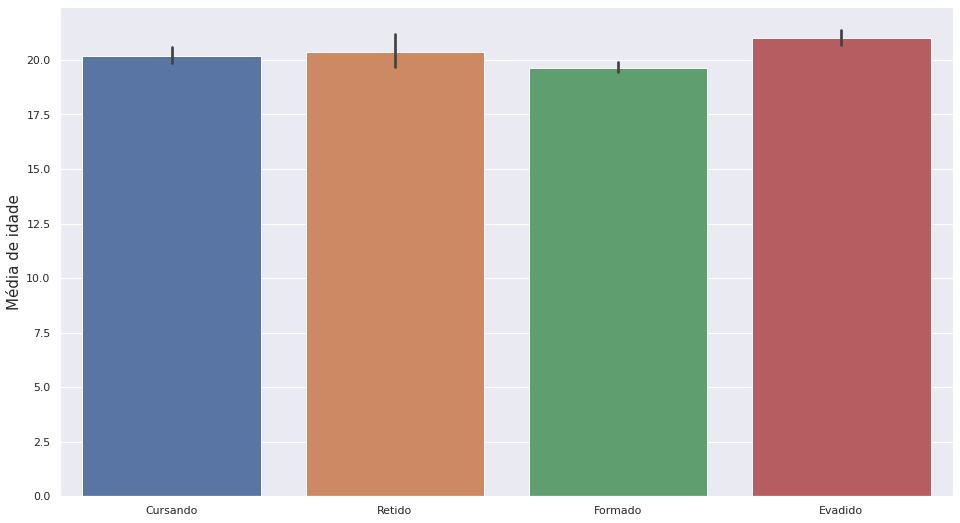
\includegraphics[scale=.45]{imagens/media-idade-situacao.png}
\caption{Média de idade dos alunos pela situação final ou atual.}
\label{fig:media-idade-situacao}
\end{figure}


\subsubsection{Idade x Média geral}

Nesta seção será apresentada uma relação entre a idade com a média geral do aluno.

\begin{figure}[htbp]
\centering 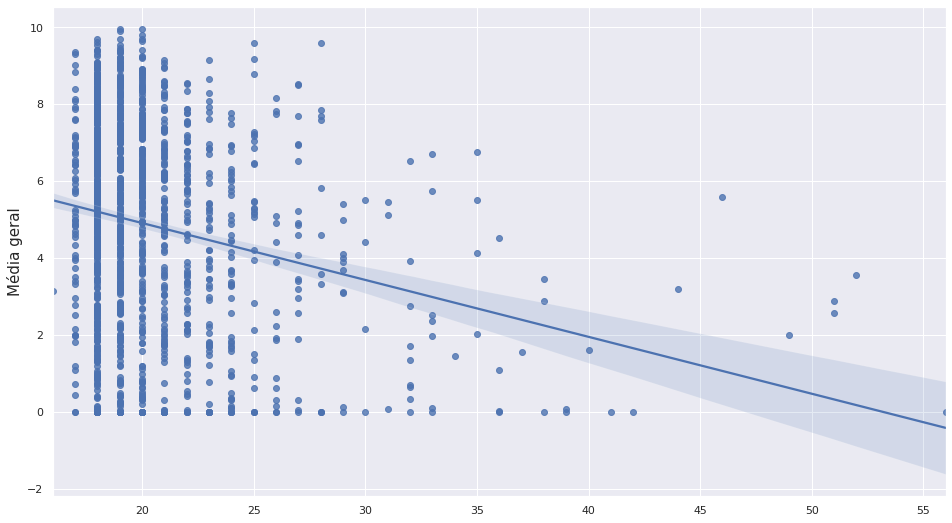
\includegraphics[scale=.45]{imagens/media-geral-idade.png}
\caption{Número de alunos por idade de ingresso no curso.}
\label{fig:media-geral-idade}
\end{figure}

A figura \ref{fig:media-geral-idade} mostra a relação entre a média geral do aluno com a idade e traça a regressão linear entre as duas.
A linha da regressão linear mostra que conforme a idade aumenta a média geral do aluno diminui.

\begin{figure}[htbp]
\centering 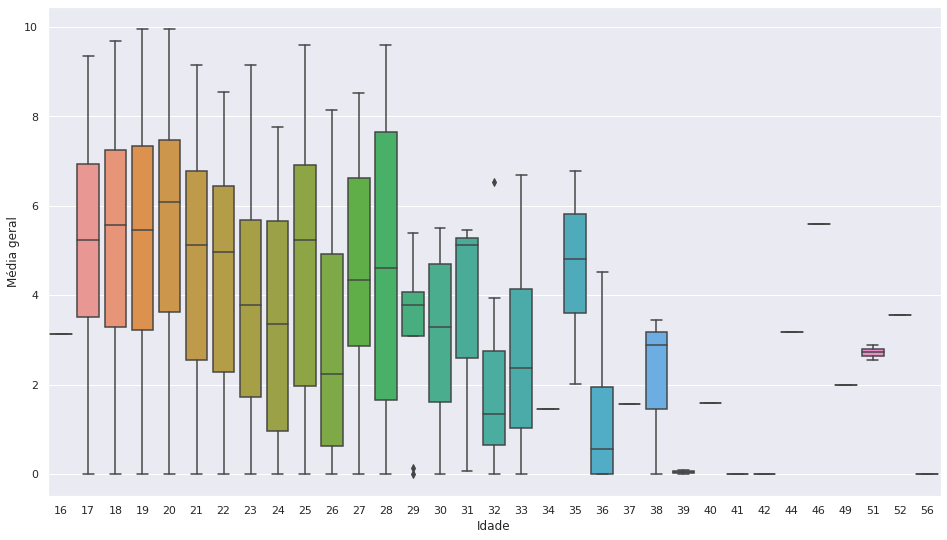
\includegraphics[scale=.43]{imagens/media-geral-idade-grafico-quartis.png}
\caption{Número de alunos por idade de ingresso no curso.}
\label{fig:media-geral-idade-grafico-quartis}
\end{figure}

A figura \ref{fig:media-geral-idade-grafico-quartis} apresenta um gráfico que expõe informações como máximo, mínimo, quartil e \textit{outlier} da média geral do aluno pela idade. A partir deste gráfico é possível verificar que o conjunto de dados possui alguns \textit{outliers} que devem ser removidos na etapa de limpeza dos dados. Nas idades onde não os mínimos, máximos e quartis significa que existem penas um ou nenhum valor para aquela idade e é apresentado apenas um traço.

% A figura \ref{fig:alunos-por-idade-de-ingresso} apresenta o número de alunos pela idade que ele tinha quando ingressou no curso e essa contagem é agrupada pela situação final ou atual desse aluno no curso.
% Os dados desse gráfico foram a partir dos quartis do atributo idade do aluno.
% % Não achei referência em livro para isso li no iste abaixo
% % http://www.dicas-spss.com/?cat=18
% Fazer uma análise dos quartis é a melhor forma de obter dados corretos quando pretendemos reorganizar uma variável de escala em classes.


% \begin{figure}[htbp]
% \centering 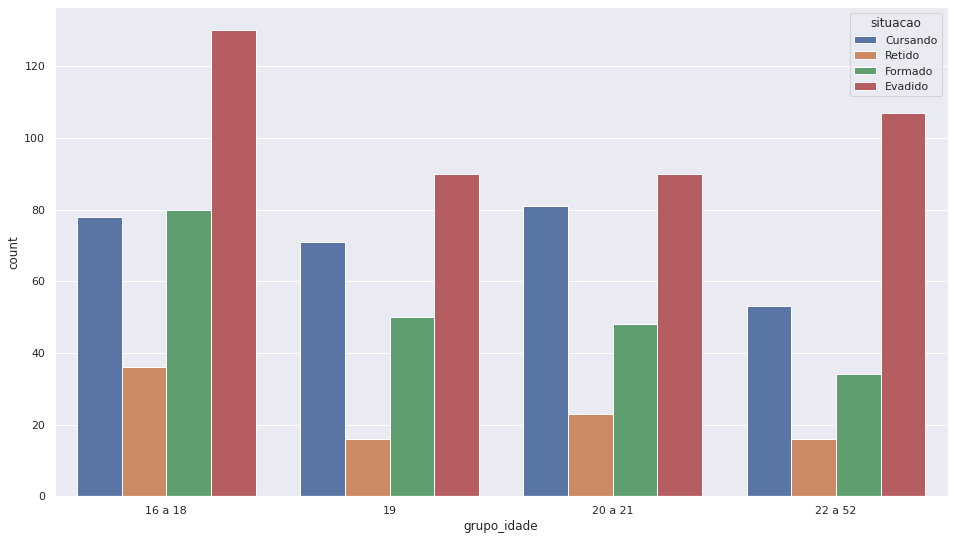
\includegraphics[scale=.5]{imagens/alunos-por-idade-de-ingresso.png}
% \caption{Número de alunos por idade de ingresso no curso.}
% \label{fig:alunos-por-idade-de-ingresso}
% \end{figure}

\subsubsection{Período de ingresso x Situação}

A figura \ref{fig:nr-alunos-ano-ingresso} apresenta uma série histórica do curso de Ciência da Computação.
O eixo x representa o ano e semestre de ingresso do aluno e o eixo y o número de alunos no período agrupados pela situação final do aluno.

\begin{figure}[!htbp]
\centering 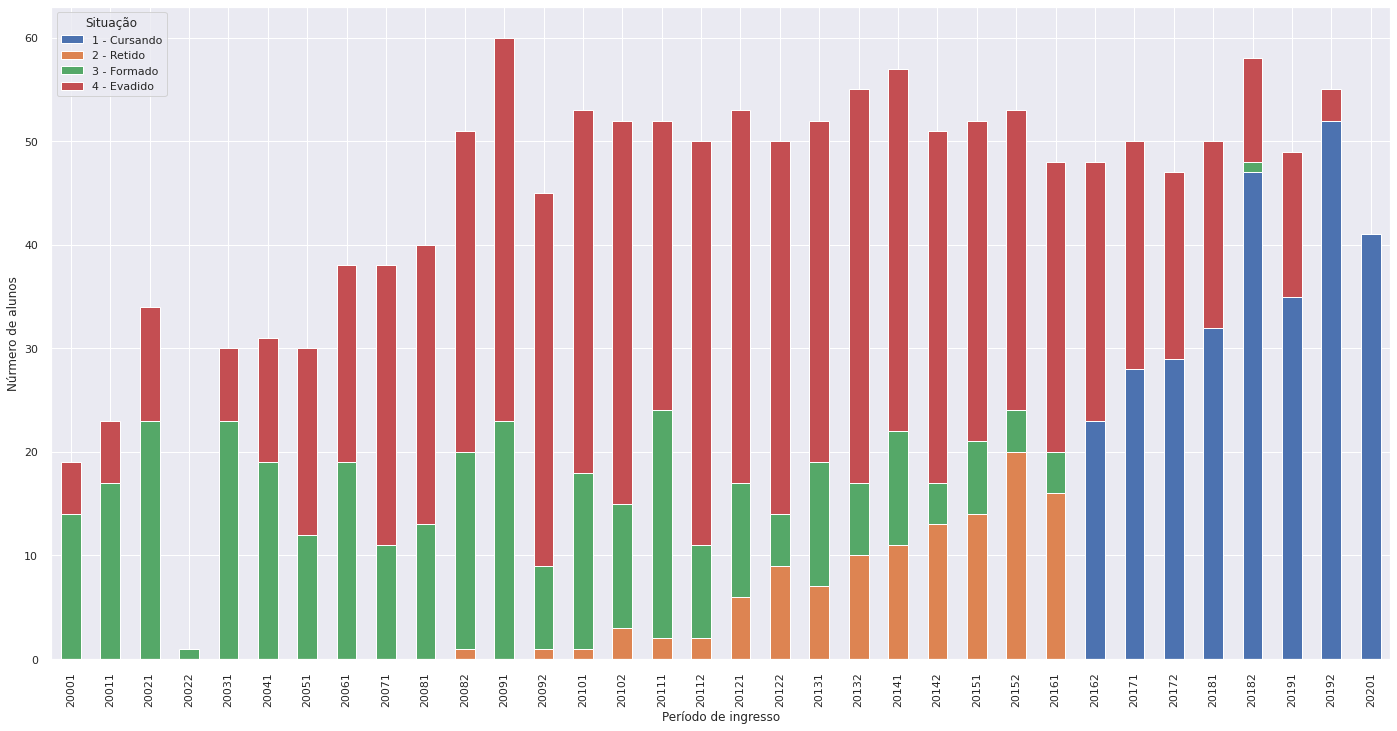
\includegraphics[scale=.32]{imagens/nr-alunos-por-perido-de-ingresso-e-situacao.png}
\caption{Número de alunos e respectiva situação pelo período de ingresso.}
\label{fig:nr-alunos-ano-ingresso}
\end{figure}

De 2000 até 2007 o curso tinha uma população de alunos formados maior do que a de alunos que evadiram.
Depois de 2007 o número de alunos formados começa a ser inferior ao número de evadidos, além disso o número de alunos retidos fica cada vez mais significante com o passar do tempo.

\subsubsection{Semestre de saída x Situação}

A figura \ref{fig:nr-alunos-semestre-saida} apresenta o número total de alunos no semestre de saída do aluno, agrupados em conjunto a respectiva situação.
É importante notar que o número de alunos evadidos diminui ao passo que o semestre aumenta.
Outro ponto que vale destacar é que o número de alunos formados cresce significativamente a partir do oitavo semestre e chega ao ponto mais alto no décimo semestre.
Isso se deve ao período de integralização curricular que em alguns currículos foi de 8 semestres e outros de 9 semestres.
Ainda é possível destacar que 19,33\% evade até o terceiro semestre e 32,45\% depois do terceiro semestre.

\begin{figure}[htbp]
\centering 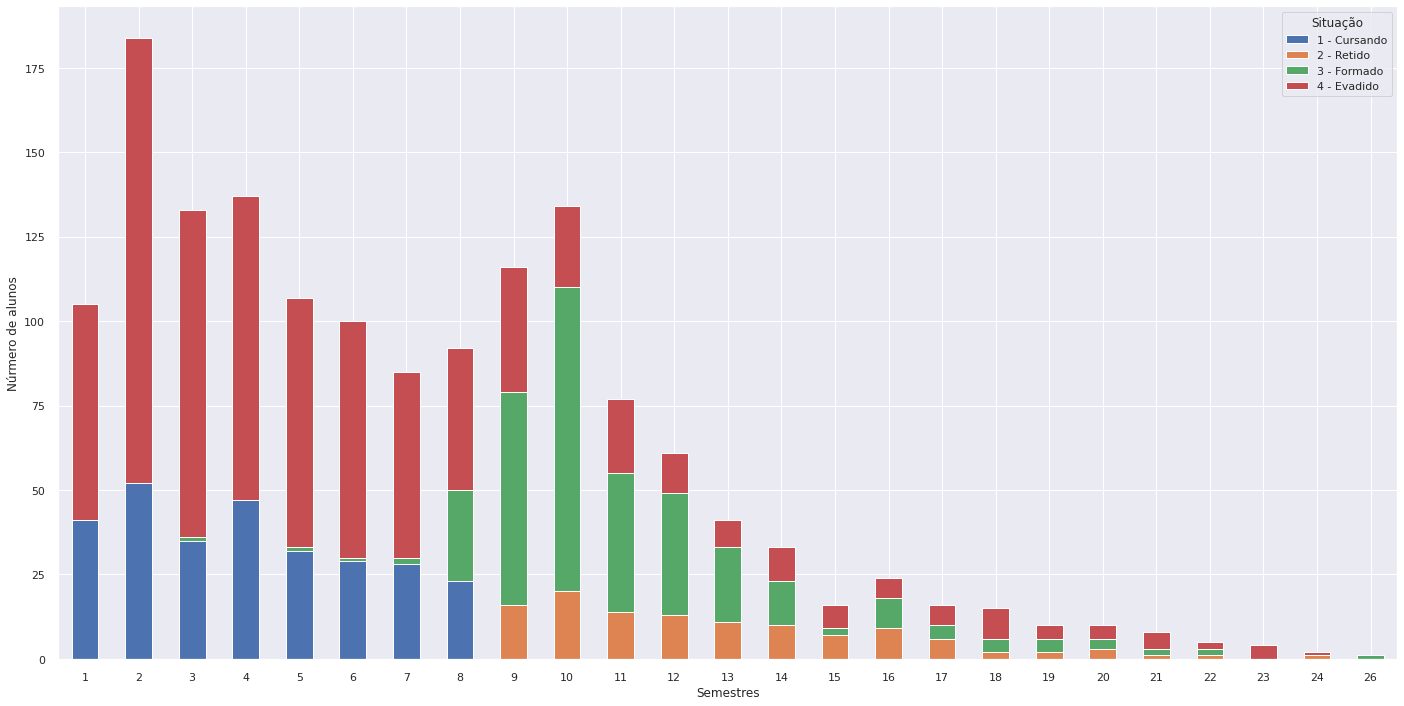
\includegraphics[scale=.32]{imagens/nr-alunos-por-semestre-e-situacao.png}
\caption{Número de alunos e respectiva situação pelo semestre de saída do aluno.}
\label{fig:nr-alunos-semestre-saida}
\end{figure}

\subsubsection{Média geral x Semestre}

A figura \ref{fig:media-geral-por-semestre} mostra a média geral dos alunos por semestre.

\begin{figure}[htbp]
\centering 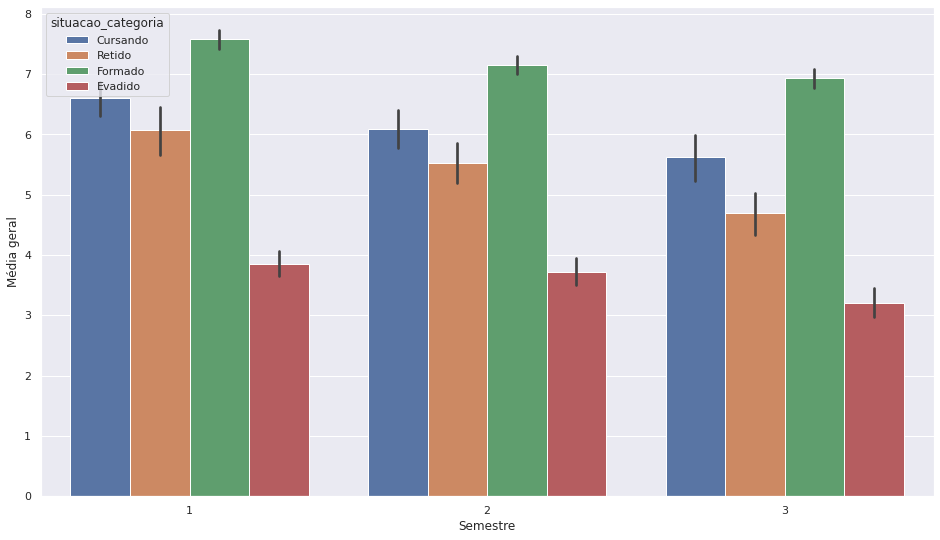
\includegraphics[scale=.45]{imagens/media-geral-por-semestre.png}
\caption{Número de alunos e respectiva situação pelo semestre de saída do aluno.}
\label{fig:media-geral-por-semestre}
\end{figure}

\section{Preparação dos dados}
\label{sec:preparacao-dados}

Nesta seção será descrito como foi feito a seleção, limpeza, formatação dos dados para a fase de modelagem dos dados. Esta seção será dividida em Seleção, Limpeza, Formatação, Criação e Descrição do conjunto final de dados, onde será descrito o que foi feito em cada uma dessas etapas.

% As etapas de modelagem e avaliação serão tradas nos capítulos de experimentos e discussões dos resultados respectivamente.


\subsection{Seleção}

Após a fase de compreensão dos dados iniciou-se a de preparação dos dados, nesta fase primeiro foi feita a seleção dos dados. Geralmente a seleção de dados tem dois enfoques distintos redução de dados horizontal e vertical \cite{goldschmidt2015data}.

A redução de dados horizontal normalmente se escolhe qual caso vai ser dado atenção.
Neste enfoque foi escolhido o curso de Ciência da Computação.

Já a redução de dados vertical visa escolher o conjunto de atributos mais relevantes para alcançar o objetivo.
Neste enfoque foram escolhidos os atributos apresentados na seção \ref{subsec:descricao-dos-dados}.
A escolha dos atributos foi baseada nos atributos de trabalhos encontrados em trabalhos relacionados.

\subsection{Limpeza}

A fase de limpeza de dados envolve verificar as informações inconsistentes, correções de erros e preencher ou eliminar valores desconhecidos e redundantes, e também retirar valores que não fazer parte do domínio em estudo \cite{goldschmidt2015data}. Em geral se faz a limpeza de informações ausentes, limpeza de inconsistências e limpeza de valores não pertencentes ao domínio.

\subsubsection{Limpeza de informações ausentes}

Neste passo os valores ausentes são eliminados do conjunto de dados.
Foram eliminados os valores ausentes dos atributos flg\_escola\_publica, nota\_final, dt\_nascimento, dt\_ingresso, naturalidade.

O atributo cota é um caso a parte, pois estão sendo avaliados dados de alunos que entraram entre 2000 e 2020, e o primeiro registro de cota aconteceu em 2014/1. Para manter este atributo todos os registros anteriores a este período foram considerados de alunos que entraram por ampla concorrência.

Antes de eliminar os valores ausentes o conjunto de dados contava com 21.105 registros de 1.514 alunos.
Após essa remover os valores ausentes ficaram 13.492 registros de 1.085 alunos.

Existem alguns métodos de preenchimento de valores tais como preenchimento manual, preenchimento com medidas estatísticas, dentre outros.
Mas esses métodos tem um custo para o desempenho final dos modelos e não forma utilizados.

\subsubsection{Limpeza de inconsistências}

Esta função tem como objetivo identificar e eliminar valores inconsistentes do conjunto de dados \cite{goldschmidt2015data}.
A inconsistência pode envolver um registro apensas ou um conjunto de registros e eles podem ser removidos ou corrigidos.

Um exemplo que aconteceu no conjunto de dados deste trabalho foi a disciplina dispensada, onde todas as disciplinas na situação dispensado não deveriam conter a nota final do aluno na disciplina, mas neste caso havia uma disciplina com nota final e na situação dispensada.

Outro exemplo foi o atributo que determina se o aluno veio de escola publica ou não. Este atributo deveria conter o valor ``S'' para alunos que vieram de escola pública e ``N'' para alunos que não vieram de escolas públicas, mas foram encontrados os valores ``P'' e ``V''. Os dois últimos valores pertenciam ao sistema anterior ao Cobalto e descobriu-se que o valor ``P'' equivale a alunos que vieram de escolas públicas e o valor ``V'' equivale a alunos que não vieram de escolas públicas.

Após a execução dessa função foi removido apensa um registro e o número total de alunos se manteve o mesmo da função anterior.

\subsubsection{Limpeza de valores que não pertencem ao domínio}

Esta função compreende a busca e eliminação de valores que não pertençam ao domínio dos atributos do problema \cite{goldschmidt2015data}. 
Ela pode ser considerada um caso particular da função de limpeza de inconsistências e é preciso ter um conhecimento prévio do problema.
Um exemplo deste trabalho foram os ``Alunos com vínculo'' que fogem do objetivo deste trabalho, pois não da para determinar se eles evadiram ou não.

Após finalizar esta função sobraram 9.725 registros de 756 alunos do conjunto de dados total. Este também foi o conjunto final de dados da fase de limpeza dos dados.

\subsection{Construção de atributos}
\label{subsec:construcao-de-atributos}

A operação de construção de atributos consiste em criar novos atributos a partir de atributos existentes. Estes novos atributos costumam ser chamados de atributos derivados  \cite{goldschmidt2015data}.
Exemplos deste trabalho foram idade, semestre que o aluno cursou uma determinada disciplina, médias do primeiro, segundo e terceiro semestre, média dos três primeiros semestres, coeficiente de ralação do primeiro, segundo e terceiro semestre, e a média do número de disciplina cursadas no três primeiros semestres.
Esses atributos foram gerados para tentar contextualizar melhor os dados retirados do sistema e obter um melhor desempenho dos algoritmos de classificação.

A idade foi gerada a partir da data de ingresso do aluno e a data de nascimento.
Foram extraídos o ano das datas e subtraído o ano da data de ingresso pelo ano da data de nascimento, e os meses e dias foram desconsiderados para fazer este cálculo.

O atributo que representa o semestre que o aluno cursou uma determinada disciplina foi gerado através de uma fórmula usando o ano/semestres de ingresso e ano/semestre que o aluno cursou a disciplina.

\[semestre = 2(ano\_dis - ano\_ing) + (sem\_dis - sem\_ing) + 1\]

Onde ano\_dis e sem\_dis correspondem ao ano e semestre que o aluno cursou a disciplina respectivamente, e ano\_ing e sem\_ing correspondem ao ano e semestre que o aluno ingressou no curso também respectivamente.

As médias do primeiro, segundo e terceiro semestre foram geradas utilizando a técnica de \textit{pivot table}, que reorganiza os valores da tabela criando novas estatísticas.
Estes atributos foram gerados utilizando o método \textit{pivot\_table} do Pandas, que é uma biblioteca do Python que faz diversas manipulações de dados. Após a execução dessa função o conjunto de dados ficou com 756 registros de 756 alunos, pois o método \textit{pivot\_table} calculou a média do primeiro, segundo e terceiro semestres em colunas do conjunto de dados.

No mesmo processo que criou as médias do primeiro, segundo e terceiro semestres foram criados o número total de disciplinas aprovadas no primeiro, segundo e terceiro semestres, através dos atributos flg\_pri\_sem, flg\_seg\_sem e flg\_ter\_sem que indicam se a disciplina pertence e foi cursada no primeiro, segundo e terceiro semestres respectivamente.

O coeficiente de ralação de cada um dos 3 primeiros semestre é dada pela razão entre o número de disciplinas aprovadas no semestre pelo o número total de disciplinas que o currículo possui no respectivo semestre. No final foram criados 3 coeficientes de ralação, um para cada semestre.

O atributo evadiu que será o atributo-alvo dos modelos de classificação foi gerado a partir da situação final ou atual do aluno.
Alunos com situação final de ``Formado'' recebeu o valor falso e o aluno com a situação diferente dessa recebeu o valor verdadeiro.

\subsection{Codificação dos dados}

A codificação dos dados é uma operação que modifica o domínio de valores de um determinado atributo.
O importante é que os dados sejam codificados para melhor suprir as limitações de determinado algoritmos de MD \cite{goldschmidt2015data}. Um exemplo seria uma rede neural que necessita que os dados estejam representados em formato numérico.

O tipo de conhecimento que se deseja buscar é fortemente influenciado pela maneira que a informação é codificada \cite{goldschmidt2015data}. Uma codificação pode ser de numérica para categórica ou vice-versa. Neste trabalho foi feito tanto uma codificação numérica para categórica, quanto uma codificação categórica para numérica.

\subsubsection{Numérica para categórica}

A codificação numérica para categórica foi feita no atributo idade, onde foi utilizado uma abordagem de mapeamento de intervalos, que também é conhecida como discretização.
As idades foram agrupadas em 5 categorias até 17, de 18 a 20, de 21 a 23, de 24 a 26 e de 27 a 56 anos.
Os intervalos foram definidos de forma arbitrária.

\subsubsection{Categórica para numérica}

A codificação categórica para numérica faz a representação dos valores categóricos em valores numéricos.
Um exemple desse tipo de representação é a representação binária padrão onde cada categoria é transformada em um valor binário.

Neste trabalho foi usado uma variação desse tipo de codificação que é chamado em inglês de \textit{dummy}.
Dummy transforma um atributo categórico em tantos atributos quanto categorias que existem no atributo e cada atributo gerado vai ter o valor 0 ou 1.
Por exemplo, o atributo gênero que no caso do sistema pode ser masculino e feminino, seriam criados dois atributos masculino e feminino onde quando um deles for 1 o outro é 0 e vice-versa. Portando uma pessoa do gênero masculino teria o atributo masculino igual a 1 e atributo feminino igual a 0.

\subsection{Conjunto final de dados}

Após todo o processo de preparação dos dados o conjunto de alunos do estudo se limitou a 756 alunos e 30 atributos socioeconômico e acadêmico que foram selecionados para o estudo.
Destes alunos, 67,5\% (513) estavam na situação de evasão do curso e um total de 32,5\% (247) estavam na situação de conclusão do curso de 2000 a 2020.

\begin{table}[htbp]
\footnotesize\addtolength{\tabcolsep}{-3pt}
\begin{center}
\caption{Relação de atributos selecionados.}\label{alunos-atributos}
\begin{tabular}{l|l}
\hline
Atributo             & Descrição                                \\
\hline
med\_1\_sem & valor \\
med\_2\_sem & valor \\
med\_3\_sem & valor \\
med\_3\_pri\_sem & valor \\
apr\_curr\_sem\_1 & valor \\

apr\_curr\_sem\_2 & valor \\
apr\_curr\_sem\_3 & valor \\
evadiu & valor \\
genero\_F & valor \\
genero\_M & valor \\

cota\_N & valor \\
cota\_S & valor \\
flg\_escola\_publica\_N & valor \\
flg\_escola\_publica\_P & valor \\
flg\_escola\_publica\_S & valor \\

flg\_escola\_publica\_V & valor \\
flg\_curso\_superior\_N & valor \\
flg\_curso\_superior\_S & valor \\
flg\_beneficio\_N & valor \\
flg\_beneficio\_S & valor \\

naturalidade\_ESTADO & valor \\
naturalidade\_MESOPELOTAS & valor \\
naturalidade\_MICROPELOTAS & valor \\
naturalidade\_PAIS & valor \\
naturalidade\_PELOTAS & valor \\

idade\_ate\_17 & valor \\
idade\_de\_18\_a\_20 & valor \\
idade\_de\_21\_a\_23 & valor \\
idade\_de\_24\_a\_26 & valor \\
idade\_de\_27\_a\_56 & valor \\
\hline
\end{tabular}
\end{center}
\end{table}

\section{Modelagem}

Esta seção corresponde a fase de Modelagem da metodologia proposta no capítulo~\ref{cap:metodologia}.
Nesta fase os algoritmos de aprendizagem de máquina (AM) são aplicados ao conjunto de dados extraído do sistema acadêmico da universidade.

Este trabalho será dividido em 3 etapas que vão descrever as ferramentas e algoritmos que foram utilizados neste trabalho.

\subsection{Etapa 1}

Na fase inicial deste trabalho foram buscadas ferramentas de fácil utilização em vista de otimizar o tempo. Nesta fase foi utilizada a ferramenta RapdiMiner Studio na versão 9.7 que é um designer de fluxo de trabalho visual para análise preditiva que traz ciência de dados e aprendizado de máquina.

O RapdiMiner Studio na versão 9.7 é possível acelerar o processo de aprendizagem e construção de modelos utilizando as abordagens guiadas \textit{Turbo Rep}, \textit{Auto Model} e \textit{Deployments}. Neste trabalho optou-se pela abordagem \textit{Auto Model}, por passar por todo o processo de mineração de dados.

O \textit{Auto Model} é um processo dividido em 6 passos \textit{Load Data}, \textit{Select Task}, \textit{Prepare Target}, \textit{Select Inputs}, \textit{Model Types} e \textit{Results}.

O primeiro passo é o \textit{Load Data}, que  é onde o conjunto de dados é carregado. Existe diversas forma de carregar os dados nesta versão do RapdiMiner e para este trabalho foi escolhida a de importar do computador local. Nesta etapa foram feitos testes com os dados do curso de Geoprocessamento e de Ciência da Computação.

Em seguida vem o passo \textit{Select Task}, que é onde tem que selecionar o tipo de tarefa de mineração de dados será realizada. A versão utilizada neste trabalho oferece 3 tipos de tarefas \textit{Predict}, \textit{Clusters} e \textit{Outiers}. Foi utilizada a tarefa \textit{Predic}, que faz a predição de uma coluna do conjunto de dados. A coluna utilizada para fazer a predição foi a de ``evasao'' que pode ser ``S'' quando o aluno evadiu e ``N'' caso tenho se formado.

No passo \textit{Prepare Target} serão dado algumas opções com relação ao atributo alvo. Uma delas é o \textit{Class of Highest Interest}, que permite selecionar a classe que os algoritmos devem focar os resultados. Isso é importante pois valores de desempenho como \textit{Precision} e \textit{Recall} precisam saber qual classe devem interpretar como resultado positivo. No caso deste trabalho é a classe ``S'', pois ela indica que o aluno evadiu do curso.

O próximo passo é \textit{Select inputs}, que ajuda selecionar os atributos que vão melhorar o desempenho dos modelos. Um ponto importante é que se procura padrões nos dados e se não tiver variações neles eles não serão uteis. Esse passo ajuda a identificar atributos que tenham uma correlação muito alto com o atributo alvo, que tenham todos ou quase todos os valores diferentes ou idênticos, ou que tenham valores faltando. Esses atributos problemáticos serão identificados e marcados, para serem agregados ou não ao conjunto de dados final.

Em \textit{Model Types} é onde seleciona os modelos que serão usados. A versão 9.7 do \textit{RapidMiner} disponibiliza 8 modelos \textit{Naive Bayes}, \textit{Generalized Linear Model}, \textit{Logistic Regression}, \textit{Deep Learning}, \textit{Decision Tree}, \textit{Random Forest}, \textit{Gradient Boosted Trees (XGBoost)}, \textit{Support Vector Machine (SVM)}. Neste trabalho os dados, tando da Ciência da Computação quanto do Geoprocessamento, foram submetidos aos 8 modelos de aprendizagem de máquina. A figura~\ref{fig:processo-rapidminer} mostra a estrutura do processo que foi gerada após finalizar o \textit{Auto Model}.

\begin{figure}[htbp]
\centering 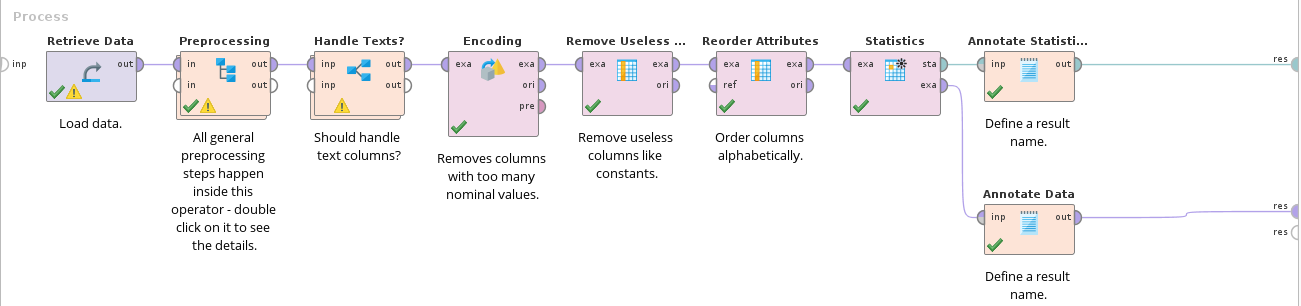
\includegraphics[scale=.35]{imagens/processo-rapidminer.png}
\caption{Estrutura do processo no RapidMiner versão 9.7.}
\label{fig:processo-rapidminer}
\end{figure}

Após executar os modelos são mostrados os resultados que é a ultima fase do \textit{Auto Model}. Nesta fase são mostrado os resultados dos modelos, como por exemplo: \textit{Accuracy, AUC, Precision, Recall, F-Measure, Sensitivity, Specificity}, dentre outras formas de avaliar os resultados dos modelos.

\subsection{Etapa 2}
\label{subsec:etapa2}

A implementação dessa etapa foi aprovada no LACLO 2020 e EMPOS 2020 e usando Python e Sklearn. Sklearn é uma biblioteca desenvolvida em Python, que possui diversas ferramentas de aprendizagem de máquina. Esta implementação foi separada em dois módulos, onde um fez a preparação dos dados e outro que submeteu os dados aos algoritmos de aprendizagem de máquina.

A preparação dos dados seguiu um roteiro que é normalmente utilizado em Ciência de Dados que é: seleção, limpeza, formatação e transformação. Foram selecionados 18 atributos e dados de 756 alunos do curso de Ciência da Computação. Destes alunos 67,5\% (513) estavam na situação de evasão do curso e um total de 32,5\% (247) estavam na situação de conclusão do curso de 2000 a 2020.

Para submeter os dados aos modelos os dados foram separados em um conjunto de treinamento e outro de testes, na proporção  de  3/4  para  treinamento  e o  restante  para  testes  utilizando \textit{train\_test\_split}.  Após  essa separação os dados de treinamento foram balanceados para tentar reduzir a quantidade de falsos negativos, que é quando os  algoritmos  predizem  que  o  aluno  não  vai  evadir,  mas na verdade ele evadiu.  Por  fim,  os  dados  foram submetidos a três algoritmos de AM, sendo eles \textit{Logistic Regression}, \textit{Decision Tree} e \textit{RandomForest}.

O trabalho apresentado no LACLO 2020 e EMPOS 2020 tiveram resultados relevantes tais como foi possível prever alunos em risco de evasão com uma acurácia de 91,05\% para o melhor resultado e que o atributo mais influenciou a predição foi a média do terceiro semestre que se destacou no \textit{feature importance} de dois dos 3 algoritmos. A tabela~\ref{tab:resultados-algoritmos-laclo-empos} apresenta os resultados alcançados nos trabalhos apresentados no LACLO 2020 e EMPOS 2020.

\begin{table}[htbp]
\footnotesize\addtolength{\tabcolsep}{-4pt}
\begin{center}
\caption{Resultados da execução dos algoritmos do LACLO 2020 e EMPOS 2020.}
\label{tab:resultados-algoritmos-laclo-empos}
\begin{tabular}{p{4cm}p{2cm}p{2cm}p{2cm}p{2cm}p{2cm}} \hline
Algoritmo           & Accuracy & Precision & Recall  & F1-score & AUC     \\ \hline
Logistic Regression & 90,00\%  & 95,80\%   & 89,06\% & 92,31\%  & 90,50\% \\
Decision Tree       & 87,37\%  & 91,94\%   & 89,06\% & 90,48\%  & 86,47\% \\
Random Forest       & 91,05\%  & 95,12\%   & 91,41\% & 93,23\%  & 90,86\% \\ \hline
\end{tabular}
\end{center}
\end{table}


\subsection{Etapa 3}

A etapa 3 é a principal etapa da metodologia é nessa etapa que acontece a busca efetiva por conhecimento.
A execução dessa etapa é a aplicação efetiva de algoritmos sobre os dados na tentativa de extrair conhecimento \cite{goldschmidt2015data}.
Neste trabalho foi feito uma abordagem de aprendizado supervisionado, onde a entrada é um conjunto de valores de uma ou mais variáveis e a saída é o valor do atributo alvo.

Nesta etapa foram utilizados 5 algoritmos, os 3 da seção \ref{subsec:etapa2}, mais Naive Bayes e Redes Neurais, também foi utilizado o método de validação cruzada estratificada.
As ferramentas utilizadas foram Python e a bibliotéca Sklearn do Python.

Para o algoritmo de \textit{Decision Tree} foi utilizado o método ``DecisionTreeClassifier'' da biblioteca Sklearn.
O método foi executado com os valores padrões do método.
Foi configurado com a estratégia Gini Impurity para medir a qualidade da divisão e \textit{Best} para a estratégia de escolher a divisão em cada nó.
Outra configuração foi a da profundidade máxima da arvore, que foi a de expandir os nós até que todas as folhas contenham menos do que 2 filhos.

O método ``RandomForestClassifier'' do módulo ``ensemble'' do Sklearn foi utilizado para implementar o classificador \textit{RandomForest}.
O método também foi mantido em sua configuração padrão que utiliza o \textit{Gini Impurity} e profundidade máxima da arvore de nenos do que 2 filhos.

O modelo de \textit{Logistic Regression} foi implementado pelo método ``LogisticRegression'', que se encontra no módulo \textit{``linear\_model''} do Sklearn.
O método foi utilizado com as configurações padrões da versão 0.23.2 da bibliotéca Sklearn.

Para implementar o modelo de Rede Neural foi utilizada o método ``MLPClassifier'' do módulo ``neural\_network'' do Sklearn. Foram utilizadas todas as configurações padrões do método ``MLPClassifier''.

A implementação do modelo Naive Bayes foi através do método ``GaussianNB'' do módulo ``naive\_bayes'' da bibliotéca Sklearn.
Assim como os outros foram mantidas as configurações padrões.

As configurações completas de cada método será coloca no anexo X deste trabalho.


\section{Conclusão do capitulo}

Este capítulo apresentou a metodologia utilizada para o desenvolvimento deste trabalho. Esta metodologia pegou como base a metodologia CRISP-DM.

Foi mostrado como foi feito compreensão dos dados apresentando cada atributo utilizado, junto com uma análise exploratória dos dados. Em seguida foi mostrado todo o processo de preparação dos dados que iniciou na seleção, até obter o conjunto final de dados. Por fim foi mostrado as 3 fase de modelagem que este trabalho passou, para chegar na configuração final.

\chapter{Experimento e Resultados}

% Estudo de caso do curso de Ciência da Computação e Engenharia.
Este capítulo corresponde a fase de avaliação da metodologia proposta no capítulo~\ref{cap:metodologia}.
Nesta fase os resultados dos algoritmos de AM serão avaliados.
Essa avaliação será dada no sentido de tentar responder as questões de pesquisa já citadas.

Este capítulo será divido em 4 seções, para tentar apresentar os resultados alcançados neste trabalho.
A seção de experimentos vai apresentar como foram realizados os experimentos.
A seção performance vai avaliar o desempenho alcançado em cada experimento.
Já a seção \textit{Feature importance} vai tentar apresentar os atributos com maior peso para determinar se o aluno evadiu ou não.
Por fim a seção de conclusão do capítulo que fará o fechamento deste capítulo.

\section{Experimentos}

Para alcançar os resultados deste trabalho foram realizados dois experimentos.
Os dois experimentos utilizaram dados socio-econômicos e acadêmicos dos alunos, porem a diferença ficou em qual tipo de dado acadêmico foi utilizado.

O primeiro experimento (experimento 1) utilizou o mesmo conjunto de dados utilizado no trabalho apresentado no LACLO 2020.
Neste experimento foram utilizados, como dado acadêmico, as médias dos 3 primeiros semestre do aluno.

O segundo experimento (experimento 2) também teve o mesmo conjunto de dados utilizado do trabalho apresentado no LACLO 2020, porem foram retiradas as médias dos 3 primeiros semestres e adicionado o fator de ralação apresentado na seção~\ref{subsec:construcao-de-atributos}.

Para ambos os experimentos foram mantidas as mesmas configurações dos algoritmos e utilizando a validação cruzada com 10 conjuntos estratificada.
Assim como no trabalho do LACLO 2020, houve uma preocupação para manter a identidade dos alunos anonimas.

\section{Performance}

Antes de buscar os atributos que mais influência na predição dos algoritmos é preciso obter uma boa acurácia.
É possível obter cada uma dessa métricas a partir da matriz de confusão resultante da execução dos algoritmos.

A Figura~\ref{fig:matriz-confusao-categorias} mostra a orientação utilizada para gerar a matriz de confusão dos algoritmos e mostra a posição do \textit{True Negative} (TN), \textit{False Positive} (FP), \textit{False Negative} (FN) e \textit{True Positive} (TP) na matriz.

\begin{figure}[htbp]
\centering 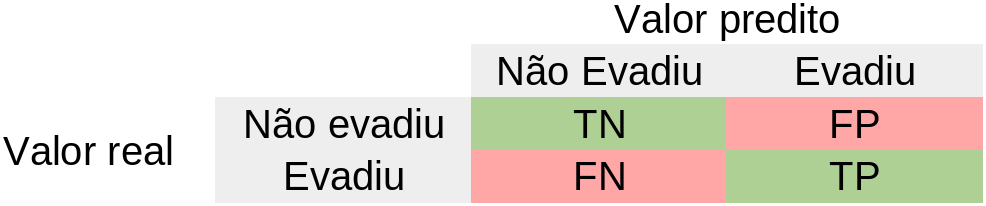
\includegraphics[scale=.4]{imagens/modelo-matriz-confusao.png}
\caption{Categorias da matriz de confusão.}
\label{fig:matriz-confusao-categorias}
\end{figure}

Para comparar os experimentos será avaliado apenas o erro, ou seja, o FP que é quando o algoritmo prevê que o aluno vai evadir mas não evade e o FN que é quando o prevê que o aluno não vai evadir mas ele evade.
O mais problemático é o FN, pois ele não classifica o aluno como um aluno que vai evadir e na verdade esse aluno evade.

A Figura~\ref{fig:matriz-confusao-arvore-decisao} mostra a matriz de confusão do experimento 1 e 2 do algoritmo de Arvore de Decisão.
O algoritmo obteve melhores resultados no experimento 1 alcançando um menor erro, com 63 FN e FP.
Enquanto que o experimento 2 alcançou o resultado de 72 FN e 78 FP, isso é 9 e 15 alunos a mais em relação ao experimento 1 respectivamente.

\begin{figure}[htbp]
\centering 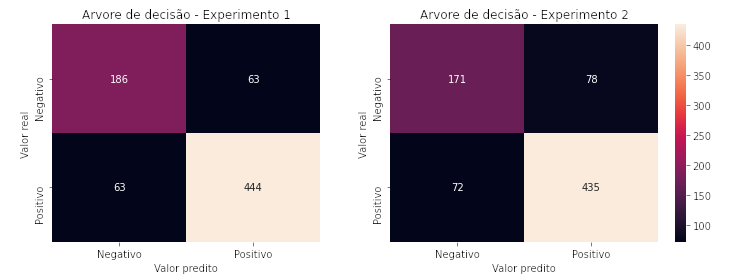
\includegraphics[scale=.62]{imagens/matriz-confusao-arvore-decisao.png}
\caption{Matriz de confusão dos experimentos 1 e 2 de Arvore de Decisão.}
\label{fig:matriz-confusao-arvore-decisao}
\end{figure}

A Figura~\ref{fig:matriz-confusao-floresta-aleatoria} mostra a matriz de confusão do experimento 1 e 2 do algoritmo de Floresta Aleatória.
Para este algoritmos os resultados foram melhores para os dados do segundo experimento, onde o FN foi de 50 alunos e o FP foi de 59 alunos.

\begin{figure}[htbp]
\centering 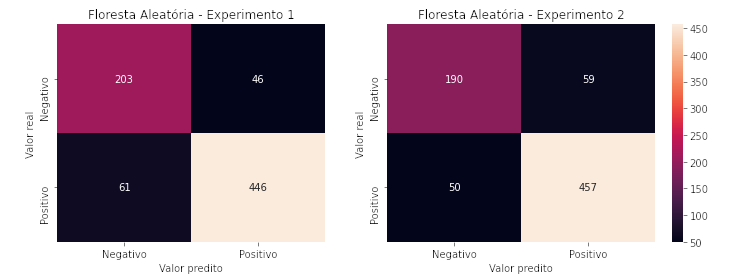
\includegraphics[scale=.62]{imagens/matriz-confusao-floresta-aleatoria.png}
\caption{Matriz de confusão dos experimentos 1 e 2 de Floresta Aleatória.}
\label{fig:matriz-confusao-floresta-aleatoria}
\end{figure}

A Figura~\ref{fig:matriz-confusao-regressao-logistica} mostra a matriz de confusão do experimento 1 e 2 do algoritmo de Regressão Logística.
Os resultados do experimento 2 para este algoritmo não foi equilibrado, pois ele obteve um FN baixo, mas o FP ficou muito alto.
Já o resultado do experimento 1 ficou mais equilibrado com 49 FN e 50 FP.


\begin{figure}[htbp]
\centering 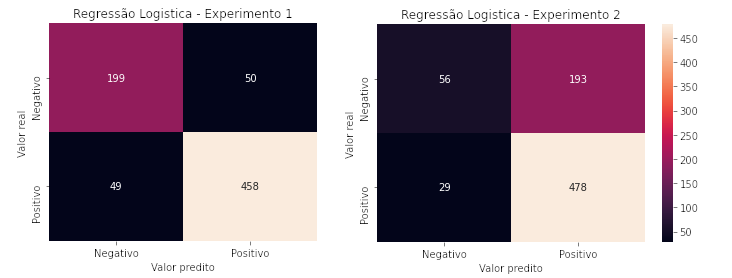
\includegraphics[scale=.62]{imagens/matriz-confusao-regressao-logistica.png}
\caption{Matriz de confusão dos experimentos 1 e 2 de Regressão Logística.}
\label{fig:matriz-confusao-regressao-logistica}
\end{figure}

A Figura~\ref{fig:matriz-confusao-redes-neurais} mostra a matriz de confusão do experimento 1 e 2 do algoritmo de Redes Neurais.
Para este algoritmo o resultado do FN foi melhor no experimento 2, mas o resultado do FP foi melhor no experimento 1.

\begin{figure}[htbp]
\centering 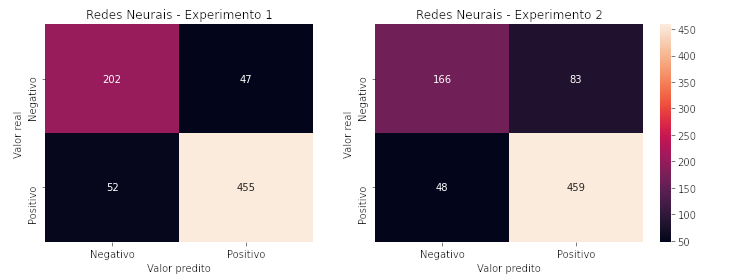
\includegraphics[scale=.62]{imagens/matriz-confusao-redes-neurais.png}
\caption{Matriz de confusão dos experimentos 1 e 2 de Redes Neurais.}
\label{fig:matriz-confusao-redes-neurais}
\end{figure}

A Figura~\ref{fig:matriz-confusao-naive-bayes} mostra a matriz de confusão do experimento 1 e 2 do algoritmo Naive Bayes.
No caso deste algoritmo o que chamou a atenção a diferença dos resultados do FP e FN do experimento 1 para os do experimento 2.

\begin{figure}[htbp]
\centering 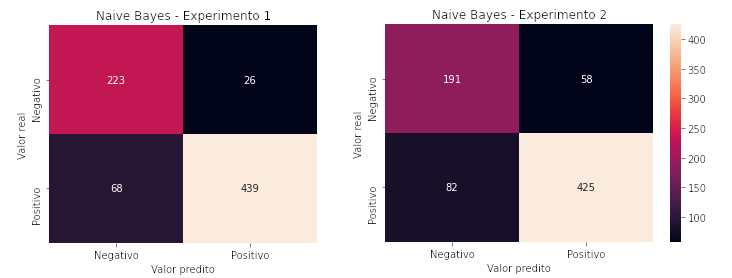
\includegraphics[scale=.62]{imagens/matriz-confusao-naive-bayes.png}
\caption{Matriz de confusão dos experimentos 1 e 2 do algoritmo Naive Bayes.}
\label{fig:matriz-confusao-naive-bayes}
\end{figure}

Deu para perceber que não é possível avaliar os resultados olhando apenas para o FP e FN.
Por isso os resultados serão avaliados pela acurácia (accuracy), precisão (precision), sensibilidade (recall) e AUC.

A acurácia é uma das métricas de modelos de ciência de dados mais utilizadas.
Em geral ela mostra o quanto o modelo está acertando.
A fórmula abaixo mostra o cálculo da acurácia utilizando os termos da matriz de confusão.

\[acur\acute{a}cia = \frac{TN + TP}{(TN + TP + FN + FP)}\]

No caso deste trabalho, utilizar a apenas a acurácia não é interessante, pois os dados estão desbalanceados. 
Nos dados obtidos do Cobalto se um modelo simplório classificasse todos os alunos como evadidos esse modelo obteria 67,5\% de acurácia, porque dos 756 alunos 513 estão em situação de evasão.

A precisão é boa para determinar quanto o custo do FP é alto.
Ele normalmente é considerada em situações em que os FPs são mais importantes do que os FNs.
Abaixo segue a fórmula da precisão.

\[precis\tilde{a}o = \frac{TP}{(TP + FP)}\]

O Recall mostra a proporção de todos os valores positivos foi identificada corretamente.
O Recall é a probabilidade do modelo predizer que o aluno evadiu dado que o aluno realmente evadiu.
Ele geralmente é utilizado em situações contrarias a da precisão, ou seja, onde FNs são considerados mais problemáticos do que os FPs.
O Recall é calculado da seguinte forma.

\[recall = \frac{TP}{(TP + FN)}\]

AUC vem do inglês \textit{Area under the ROC Curve}, para poder explicar esta métrica é preciso falar da curva ROC antes.

A curva ROC (\textit{Receiver Operating Characteristic}) é um gráfico que mostra o desempenho dos modelos de classificação.
Ela representa True Positive Rate (TPR) versus False Positive Rate (FPR) em diferentes limiares de classificação.
O TPR é equivalente ao recall e o FPR é definido como segue abaixo.

\[FPR = \frac{FP}{(FP + TN)}\]

Para calcular cada ponto da curva ROC, é possível utilizar um modelo de regressão logística modificando os limiares de classificação até gerar todos os pontos. Porem existe um algoritmo de classificação chamado AUC que a área abaixo da curva ROC.

AUC calclula a área abaixo de todos os limiares de classificação possíveis da curva ROC. Quanto mais alto é o valor do AUC melhor é a capacidade do modelo de classificação em distinguir entre as classes positivas e negativas, no caso deste trabalho se o aluno evade ou não.


A Tabela~\ref{tab:resultado-experimento-1} mostra os resultados do experimento 1, onde foi utilizado as médias dos 3 primeiro semestres.
O algoritmo que obteve a melhor AUC foi o Naive Bayes com 88,07\% e o pior foi Arvore de decisão com 81,14\%.
Em relação ao Recall o modelo que se saiu melhor foi o de Regressão logística com 90,34\% e o pior foi Naive bayes com 86,59\%. Redes neurais foi o modelo que obteve o resultado mais equilibrado obteve o segundo melhor desempenho tanto na AUC quanto no Recall.

\begin{table}[htbp]
\footnotesize\addtolength{\tabcolsep}{-3pt}
\begin{center}
\caption{Resultado da execução dos algoritmos com os dados do experimento 1.}
\label{tab:resultado-experimento-1}
\begin{tabular}{p{4cm}p{2cm}p{2cm}p{2cm}p{2cm}} 
\hline
Algoritmo           & \multicolumn{1}{l}{Accuracy} & \multicolumn{1}{l}{Precision} & \multicolumn{1}{l}{Recall} & \multicolumn{1}{l}{AUC} \\ \hline
Arvore de decisão	& 83.33\%	& 87.57\%	& 87.57\%	& 81.14\% \\
Floresta Aleatória	& 85.85\%	& 90.65\%	& 87.97\%	& 84.75\% \\
Regressão Logistica	& 86.90\%	& 90.16\%	& 90.34\%	& 85.13\% \\
Redes Neurais	    & 86.90\%	& 90.64\%	& 89.74\%	& 85.43\% \\
Naive Bayes	        & 87.57\%	& 94.41\%	& 86.59\%	& 88.07\% \\  \hline
\end{tabular}
\end{center}
\end{table}


A Tabela~\ref{tab:resultado-experimento-2} mostra os resultados do experimento 2, que utilizou o coeficiente de ralação dos 3 primeiros semestres.
A melhor AUC no segundo experimento foi do modelo de Floresta aleatória, com 83,22\%, e o pior foi o de Regressão logística, com 58,39\%.
Vale destacar que o modelo de Regressão logística teve o maior Recall para este experimento 94,28\%, porém o modelo não aprendeu pois a acurácia foi de 70,63\%, que fica 3,13\% acima de uma modelo que aposta-se sempre na evasão.

\begin{table}[htbp]
\footnotesize\addtolength{\tabcolsep}{-3pt}
\begin{center}
\caption{Resultado da execução dos algoritmos com os dados do experimento 2.}
\label{tab:resultado-experimento-2}
\begin{tabular}{p{4cm}p{2cm}p{2cm}p{2cm}p{2cm}} 
\hline
Algoritmo           & \multicolumn{1}{l}{Accuracy} & \multicolumn{1}{l}{Precision} & \multicolumn{1}{l}{Recall} & \multicolumn{1}{l}{AUC} \\ \hline
Arvore de decisão	& 80.16\%	& 84.80\%	& 85.80\%	& 77.24\% \\
Floresta Aleatória	& 85.58\%	& 88.57\%	& 90.14\%	& 83.22\% \\
Regressão Logistica	& 70.63\%	& 71.24\%	& 94.28\%	& 58.39\% \\
Redes Neurais	    & 82.67\%	& 84.69\%	& 90.53\%	& 78.60\% \\
Naive Bayes	        & 81.48\%	& 87.99\%	& 83.83\%	& 80.27\% \\ \hline
\end{tabular}
\end{center}
\end{table}




\section{Feature Importance}

Nesta seção será utilizada a técnica de Feature Importance para analisar quais são os atributos mais relevantes para o modelo que obteve melhor desempenho para cada experimento.
Esta técnica atribui uma pontuação a cada atributo com base na sua relevância para prever a variável de saída.

Para analisar a Feature Importance de um modelo é importante que este modelo tenha obtido um bom desempenho na predição, pois não teria relevância analisar a Feature Importance de modelos que não consegue fazer uma boa predição.

\subsection{Experimento 1}

Para determinar qual modelo teve o melhor desempenho foi calculado a média entre as 4 métricas da tabela~\ref{tab:resultado-experimento-1} de cada modelo e foi selecionado o que obteve a maior média.
O modelo que obteve o melhor desempenho no experimento 1 foi o de Regressão logística com a média das métricas de 88,53\%.

A figura~\ref{fig:e1-feature-importance-rl} mostra a Feature Importance do modelo de Regressão logística.
O atributo com maior relevância para prever se o aluno evadiu ou não foi a média do terceiro semestre, seguida pela média do segundo e terceiro semestre.
Outros atributos como gênero, se aluno teve curso superior anterior, e outros não tiveram muita relevância para a predição.


\begin{figure}[htbp]
\centering
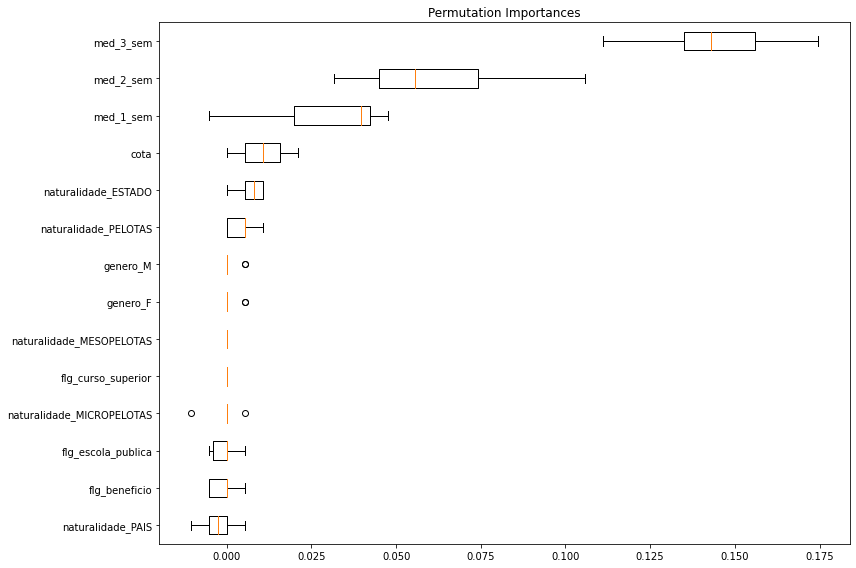
\includegraphics[scale=.53]{imagens/e1-feature-importance-rl.png}
\caption{Feature importance do modelo de Regressão logística.}
\label{fig:e1-feature-importance-rl}
\end{figure}

\subsection{Experimento 2}

Para determinar qual modelo teve o melhor desempenho, assim como no experimento 1, foi calculado a média entre as 4 métricas da tabela~\ref{tab:resultado-experimento-2} de cada modelo e foi selecionado o que obteve a maior média.
O modelo que obteve o melhor desempenho no experimento 2 foi o de Floresta aleatória com a média das métricas de 87,08\%.

A figura~\ref{fig:e2-feature-importance-rf} mostra a Feature Importance do modelo de Floresta aleatória.
Onde o atributo com maior relevância para prever se o aluno evadiu ou não foi o coeficiente de ralação do terceiro semestre, seguido pelo coeficiente de ralação do primeiro semestre.

\begin{figure}[htbp]
\centering
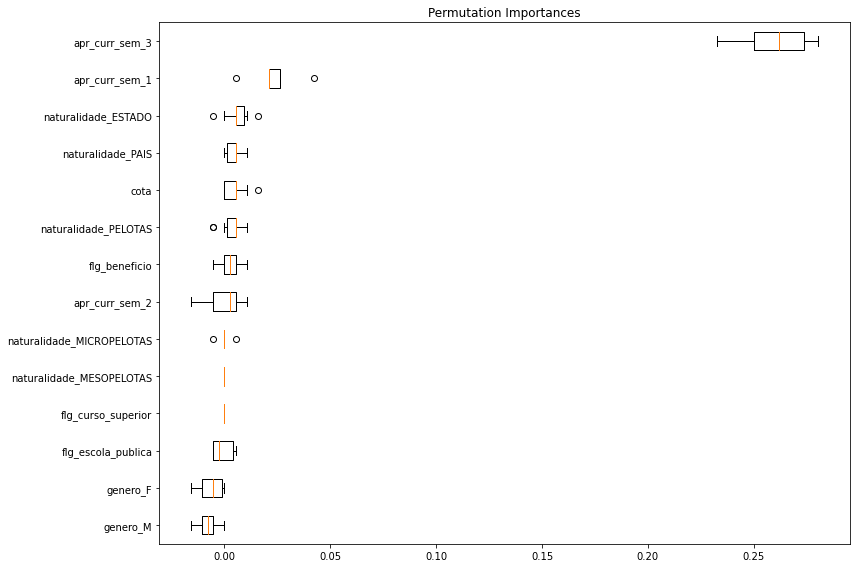
\includegraphics[scale=.53]{imagens/e2-feature-importance-rf.png}
\caption{Feature importance do modelo de Regressão logística.}
\label{fig:e2-feature-importance-rf}
\end{figure}

\section{Conclusão do capítulo}

Neste capitulo foram analisados os resultados obtidos com a execução dos modelos de aprendizado de máquina.
Os resultados foram separados em dois experimentos e analisados individualmente.
Os modelo de aprendizado de máquina foram os mesmo para ambos os experimentos.

Os resultados do experimento 1 mostraram que é possível fazer a predição de alunos em risco de evasão através das notas dos 3 primeiros semestres com uma acurácia de até 87,57\%.
Neste experimento o modelo com melhor resultado utilizando o método de avaliação foi o de Regressão logística com a média de 88,53\%.

Já o resultados do experimento 2, que usa o coeficiente de ralação, teve como melhor resultado no método de avaliação foi o modelo de Floresta aleatória.
Diferente do experimento 1, o melhor modelo não teve o melhor Recall, ficando abaixo da Regressão logística e redes neurais.

Neste trabalho foi dado uma atenção maior para o Recall, pois no contexto deste trabalho dizer que o aluno não vai evadir e esse aluno evadir é um problema mais do que o contrário.
Por exemplo, se a universidade tivesse um programa de apoio que fosse colocar os alunos com probabilidade de evadir em monitorias, isso não seria uma perda para o aluno que não fosse evadir.
Por isso o Recall é uma métrica importante neste caso e é preciso considerar ele mais que do que as outras métricas.


\chapter{Considerações Finais}

Este trabalho apresentou os resultados para a predição da evasão de alunos através de dados dos três primeiros semestres do curso de Ciência da Computação da UFPel que ingressaram entre os períodos de 2000 e 2020.
Para fazer essa classificação foi utilizado o processo de KDD e algoritmos de aprendizagem de máquina.
Os resultados mostraram que é possível prever a evasão com uma acurácia de até 87,57\%.

Neste trabalho foram elaboradas duas questão que nortearam toda a pesquisa. Uma para tentar identificar quais atributos mais influenciam no processo de evasão de alunos no curso. A outra para identificar quais modelos ou técnicas que podem ser utilizados para realizar esta tarefa.

Para responder a primeira questão de pesquisa foi utilizado os Feature Importance resultante do treinamento dos algoritmos. O experimento 1 mostrou que dados acadêmicos dos alunos influenciam na predição de alunos em risco de evasão. O experimento 2, que utilizou o coeficiente de ralação, mostrou que este atributo também é o que mais influencia na predição. Em ambos os experimentos foi possível observar que atributos como o local de nascimento do aluno e a cota também são atributos que podem influenciar na predição.

E para responder a segunda questão de pesquisa foram apresentados os resultados que os algoritmos alcançaram.
No experimento 1 o modelo que se destacou foi o de Regressão logística, que mostrou que é possível prever alunos em risco de evasão com uma acurácia de 86,90\%, e um Recall e AUC de 90,34\% e 85,13\% respectivamente.
Já o experimento 2 o modelo que mostrou que é possível predizer alunos em risco de evasão com uma acurácia de 85,58\% foi o de Floresta aleatória, que teve um Recall e AUC de 90,14\% e 83,22\% respectivamente.

Como trabalhos futuros pretende-se expandir a análise deste modelo de predição para outros cursos, primeiramente da área de exatas e engenharias e após demais cursos. Desta forma, será possível analisar a viabilidade ou não deste modelo em outros cursos e caso necessário adaptá-lo.

% Bibliografia http://liinwww.ira.uka.de/bibliography/index.html um
% site que cataloga no formato bibtex a bibliografia em computacao
% \bibliography{nomedoarquivo.bib} (sem extensao)
% \bibliographystyle{formato.bst} (sem extensao)

\bibliographystyle{abnt}
\bibliography{referencias} 


% Apêndices (Opcional) - Material produzido pelo autor
\apendices

\chapter{Um Apêndice}

% Anexos (Opcional) - Material produzido por outro
\anexos

\chapter{Um Anexo}

       \begin{table}
            % \footnotesize\addtolength{\tabcolsep}{-3pt}
            \begin{center}
                \caption{Dicionário de dados de atributos retirados do Cobalto}\label{dicionario-dados}
                \begin{tabular}{p{3cm}|p{8cm}|p{4cm}}
                    \hline
                    Atributo & Descrição & Classificação \\ \hline \hline
                    aluno\_situacao & Situação final do aluno no curso. & Quantitativa discreta \\ \hline
                    ano\_cursado e semestre\_cursado & Ano e semestre que o aluno cursou a disciplina. & Quantitativa discreta \\ \hline
                    ano\_ingresso e semestre\_ingresso & Ano e semestre que o aluno ingressou no curso. & Quantitativa discreta \\ \hline
                    ano\_saida e semestre\_saida & Ano e semestre que o aluno saiu do curso. & Quantitativa discreta \\ \hline
                    benefício & Aluno recebeu auxílio. & Qualitativa nominal \\ \hline
                    cod\_aluno & Identificador do aluno. & Quantitativa discreta \\ \hline
                    cota & Cota de ingresso do aluno. & Qualitativa ordinal \\ \hline
                    curriculo\_1 & Número de disciplinas no primeiro semestre do currículo do aluno. & Quantitativa contínua \\ \hline
                    curriculo\_2 & Número de disciplinas no segundo semestre do currículo do aluno. & Quantitativa contínua \\ \hline
                    curriculo\_3 & Número de disciplinas no terceiro semestre do currículo do aluno. & Quantitativa contínua \\ \hline
                    curriculo\_4 & Número de disciplinas no quarto semestre do currículo do aluno. & Quantitativa contínua \\ \hline
                    curso\_superior & Aluno concluiu ensino superior anterior. & Qualitativa nominal \\ \hline
                    disciplina\_situacao & Situação do aluno na disciplina. & Qualitativa ordinal \\ \hline
                    dt\_ingresso & Data de ingresso no curso. & Quantitativa contínua \\ \hline
                    dt\_nascimento & Data de nascimento do aluno. & Quantitativa contínua \\ \hline
                    escola\_publica & Aluno veio de escola pública. & Qualitativa nominal \\ \hline
                    estado\_civil & Estado civil do aluno. & Quantitativa discreta \\ \hline
                    etnia & Etnia do aluno. & Quantitativa discreta \\ \hline
                    naturalidade & Cidade natal do aluno. & Qualitativa nominal \\ \hline
                    nota\_final & Nota final do aluno em uma disciplina. & Quantitativa contínua \\ \hline
                    semestre\_1 & Número de disciplinas cursadas no primeiro semestre do currículo do aluno. & Quantitativa contínua \\ \hline
                    semestre\_2 & Número de disciplinas cursadas no segundo semestre do currículo do aluno. & Quantitativa contínua \\ \hline
                    semestre\_3 & Número de disciplinas cursadas no terceiro semestre do currículo do aluno. & Quantitativa contínua \\ \hline
                    semestre\_4 & Número de disciplinas cursadas no quarto semestre do currículo do aluno. & Quantitativa contínua \\ \hline
                    semestre\_disciplina & Semestre em que a disciplina cursada. & Quantitativa contínua \\ \hline
                    sexo & Gênero do aluno. & Qualitativa nominal \\ \hline
                    tempo\_curso & Número de semestres que o aluno cursou ou está cursando no curso. & Quantitativa contínua \\ \hline
                    tipo\_ingresso & Forma de ingresso do aluno. & Qualitativa nominal \\ \hline
                \end{tabular}
            \end{center}
        \end{table}

\chapter{Outro Anexo}

Bla blabla blablabla bla.  Bla blabla blablabla bla.  Bla blabla
blablabla bla.  Bla blabla blablabla bla.  Bla blabla blablabla bla.
Bla blabla blablabla bla.  Bla blabla blablabla bla.  Bla blabla
blablabla bla.  Bla blabla blablabla bla.  Bla blabla blablabla bla.
Bla blabla blablabla bla.  Bla blabla blablabla bla.  Bla blabla
blablabla bla.  Bla blabla blablabla bla.  Bla blabla blablabla bla.
Bla blabla blablabla bla.  Bla blabla blablabla bla.  Bla blabla
blablabla bla.  Bla blabla blablabla bla.  Bla blabla blablabla bla.
Bla blabla blablabla bla.

Bla blabla blablabla bla.  Bla blabla blablabla bla.  Bla blabla
blablabla bla.  Bla blabla blablabla bla.  Bla blabla blablabla bla.
Bla blabla blablabla bla.  Bla blabla blablabla bla.  Bla blabla
blablabla bla.  Bla blabla blablabla bla.  Bla blabla blablabla bla.
Bla blabla blablabla bla.  Bla blabla blablabla bla.  Bla blabla
blablabla bla.  Bla blabla blablabla bla.  Bla blabla blablabla bla.
Bla blabla blablabla bla.  Bla blabla blablabla bla.  Bla blabla
blablabla bla.  Bla blabla blablabla bla.  Bla blabla blablabla bla.
Bla blabla blablabla bla.

% Faz a capa do CDROM
% \makecover

\end{document}

